%!TEX program = xelatex
%!TEX options=--shell-escape
\documentclass[12pt]{article}

%
\usepackage[scheme=plain]{ctex}
%
\usepackage{fontspec}
%
\usepackage[margin = 1in]{geometry}

%
\usepackage[dvipsnames]{xcolor}
\usepackage[many]{tcolorbox}

%
\usepackage{amsmath}
\usepackage{amssymb}
\usepackage{amsthm}
%
\usepackage{tensor}
%
\usepackage{slashed}
\usepackage{physics}
\usepackage{simpler-wick}

%
\usepackage[version=4]{mhchem}

%
\usepackage{mathtools}

%
\usepackage{bm}
\newcommand{\dbar}{\dif\hspace*{-0.18em}\bar{}\hspace*{0.2em}}
\DeclareMathAlphabet\mathbfcal{OMS}{cmsy}{b}{n}
%\usepackage{bbold}
\newcommand*{\dif}{\mathop{}\!\mathrm{d}}
\newcommand*{\euler}{\mathrm{e}}
\newcommand*{\imagi}{\mathrm{i}}

\renewcommand{\vec}[1]{\boldsymbol{\mathbf{#1}}}

\usepackage{caption}
\usepackage{multirow}
\usepackage{enumitem}

%
\usepackage{mathrsfs}
\usepackage{dsfont}

%
\usepackage{hyperref}
\hypersetup{
    colorlinks=true,
    linkcolor=violet,
    filecolor=blue,      
    urlcolor=blue,
    citecolor=cyan,
}

%
\usepackage{graphicx}
\usepackage{subfig}
%
\graphicspath{{image/}}


%
\usepackage{indentfirst}
%
\setlength{\parindent}{2em}
\linespread{1.25}

% 
% \setmainfont{Times New Roman}

\title{Note}
\author{Feng-Yang Hsieh}
\date{}

\begin{document}
\maketitle

\section{SPANet2}% (fold)
\label{sec:spanet2}
	Version 2 of SPANet. call it SPANet2. 
	\subsection{Defining event topology}% (fold)
	\label{sub:defining_event_topology}
		Defining the event topology in \verb+.ymal+ file. The structure of the \verb+.yaml+ file follows this format:
		\begin{verbatim}
		INPUTS:
		    SEQUENTIAL:
		\end{verbatim}
	% subsection defining_event_topology (end)
	\subsection{Creating training dataset}% (fold)
	\label{sub:creating_training_dataset}
		\verb+.hdf5+
	% subsection creating_training_dataset (end)
	\subsection{Training options}% (fold)
	\label{sub:training_options}
		
	% subsection training_options (end)
	\subsection{Training}% (fold)
	\label{sub:training}
		Training:
		\begin{verbatim}
			python -m spanet.train -of <OPTIONS_FILE> --log_dir <LOG_DIR>  --name <NAME> 
		\end{verbatim}
		\verb+<OPTIONS_FILE>+: JSON file with options. \verb+<LOG_DIR>+: output directory. \verb+<NAME>+: subdirectory name

		Evaluation:
		\begin{verbatim}
			python -m spanet.test <log_directory> -tf <TEST_FILE>
		\end{verbatim}
		\verb+<log_directory>+: directory containing the checkpoint and options file.  \verb+<TEST_FILE>+ will replace the test file in the option file.

		Prediction:
		\begin{verbatim}
			python predict.py <log_directory> <output name> -tf <TEST_FILE> --gpu ???
		\end{verbatim}
	
	% subsection training (end)
% section spanet2 (end)
\section{Test SPANet2}% (fold)
\label{sec:test_spanet2}
	\subsection{SM SPANet}% (fold)
	\label{sub:sm_spanet}
		Generate the correct format $\kappa_\lambda = 1$ training data for SPANet2 training.
		\begin{itemize}
			\item Training sample:
			\begin{itemize}
				\item Total sample size: 76,131
				\item 1h sample size: 14,527
				\item 2h sample size: 60,122
				\item 5\% used on validation
			\end{itemize}
			\item Testing sample:
			\begin{itemize}
				\item Total sample size: 8,460
				\item 1h sample size: 1,577
				\item 2h sample size: 6,744
			\end{itemize}
		\end{itemize}
		The training results are presented in Table \ref{tab:SPANet2_diHiggs_4btag_DL1r_pt40_k1}.
		\begin{table}[htpb]
			\centering
			\caption{SPA-NET2 training results on the SM di-Higgs samples.}
			\label{tab:SPANet2_diHiggs_4btag_DL1r_pt40_k1}
			\begin{tabular}{c|c|cc}
				$N_\text{Jet}$ & Event Fraction & Event Efficiency & Higgs Efficiency \\
				\hline
				$=4$	  &   0.280             &    0.907              &    0.907             \\
				$=5$	  &   0.287             &    0.806              &    0.847             \\
				$\ge 6$	  &   0.229             &    0.679              &    0.753             \\
				Total	  &   0.797             &    0.805              &    0.841             \\
			\end{tabular}
		\end{table}

	% subsection sm_spanet (end)
	\subsection{\texorpdfstring{$\kappa 5$}{kappa 5} SPANet}% (fold)
	\label{sub:kappa_5_spanet}
		Generate the $\kappa_\lambda = 5$ training data for SPANet2 training.
		\begin{itemize}
			\item Training sample:
			\begin{itemize}
				\item Total sample size: 78,388
				\item 1h sample size: 16,013
				\item 2h sample size: 59,180
				\item 5\% used on validation
			\end{itemize}
			\item Testing sample: 
			\begin{itemize}
				\item Total sample size: 8,710
				\item 1h sample size: 1,846
				\item 2h sample size: 6,486
			\end{itemize}
		\end{itemize}
		The training results are presented in Table \ref{tab:SPANet2_diHiggs_4btag_DL1r_pt40_k5}.
		\begin{table}[htpb]
			\centering
			\caption{SPA-NET2 training results on the di-Higgs $\kappa_\lambda =5$ samples.}
			\label{tab:SPANet2_diHiggs_4btag_DL1r_pt40_k5}
			\begin{tabular}{c|c|cc}
				$N_\text{Jet}$ & Event Fraction & Event Efficiency & Higgs Efficiency \\
				\hline
				$=4$	  &   0.315             &    0.689              &    0.689             \\
				$=5$	  &   0.255             &    0.617              &    0.639             \\
				$\ge 6$	  &   0.174             &    0.499              &    0.544             \\
				Total	  &   0.745             &    0.620              &    0.638             \\
			\end{tabular}
		\end{table}

	% subsection kappa_5_spanet (end)
	\subsection{Resonant SPANet}% (fold)
	\label{sub:resonant_spanet}
		Generate the correct format resonant training data for SPANet2 training.
		\begin{itemize}
			\item Training sample:
			\begin{itemize}
				\item Total sample size: 51,145
				\item 1h sample size: 9,320
				\item 2h sample size: 40,991
				\item 5\% used on validation
			\end{itemize}
			\item Testing sample:
			\begin{itemize}
				\item Total sample size: 5,683
				\item 1h sample size: 1,011
				\item 2h sample size: 4,582
			\end{itemize}
		\end{itemize}
		The training results are presented in Table \ref{tab:SPANet2_diHiggs_4btag_DL1r_pt40_res}.
		\begin{table}[htpb]
			\centering
			\caption{SPA-NET2 training results on the resonant di-Higgs samples.}
			\label{tab:SPANet2_diHiggs_4btag_DL1r_pt40_res}
			\begin{tabular}{c|c|cc}
				$N_\text{Jet}$ & Event Fraction & Event Efficiency & Higgs Efficiency \\
				\hline
				$=4$	  &   0.316             &    0.930              &    0.930             \\
				$=5$	  &   0.282             &    0.808              &    0.839             \\
				$\ge 6$	  &   0.208             &    0.660              &    0.727             \\
				Total	  &   0.806             &    0.818              &    0.846             \\
			\end{tabular}
		\end{table}

	% subsection resonant_spanet (end)

	\subsection{Mixing \texorpdfstring{$\kappa_\lambda$}{kappa} SPANet}% (fold)
	\label{sub:mixing_kappa_spanet}
		Generate the correct format mixing $\kappa_\lambda$ training data for SPANet2 training.
		\begin{itemize}
			\item Training sample:
			\begin{itemize}
				\item Total sample size: 51,145
				\item 1h sample size: 9,320
				\item 2h sample size: 40,991
				\item 5\% used on validation
			\end{itemize}
			\item Testing sample:
			\begin{itemize}
				\item Total sample size: 5,683
				\item 1h sample size: 1,011
				\item 2h sample size: 4,582
			\end{itemize}
		\end{itemize}
		The training results are presented in Table \ref{tab:SPANet2_diHiggs_4btag_DL1r_pt40_mix}.
		\begin{table}[htpb]
			\centering
			\caption{SPA-NET2 training results on the resonant di-Higgs samples.}
			\label{tab:SPANet2_diHiggs_4btag_DL1r_pt40_mix}
			\begin{tabular}{c|c|cc}
				$N_\text{Jet}$ & Event Fraction & Event Efficiency & Higgs Efficiency \\
				\hline
				$=4$	  &   0.316             &    0.930              &    0.930             \\
				$=5$	  &   0.282             &    0.808              &    0.839             \\
				$\ge 6$	  &   0.208             &    0.660              &    0.727             \\
				Total	  &   0.806             &    0.818              &    0.846             \\
			\end{tabular}
		\end{table}

		
	% subsection mixing_kappa_spanet (end)
	\subsection{Summary}% (fold)
	\label{sub:summary}
		In most cases, the performance of SPANet2 is worse than the old one. Some default options are different between the two versions. But even if the options are set as identical, the training results also cannot be better.

		The training results of old and new versions SPANet have been summarized in Table \ref{tab:training_results_of_SPANET_12}.
		\begin{table}[htpb]
			\centering
			\caption{SPA-NET2 training results on the resonant di-Higgs samples.}
			\label{tab:training_results_of_SPANET_12}
			\begin{tabular}{c|cc}
						 & \multicolumn{2}{c}{Event efficiency} \\
						 & SPANet           & SPANet2           \\ \hline
			SM           & 0.868            & 0.805             \\
			kappa 5      & 0.725            & 0.620             \\
			Resonant     & 0.903            & 0.818             \\
			Mixing $\kappa_\lambda$& 0.833            & 0.830            
			\end{tabular}
		\end{table}

	% subsection summary (end)

% section test_spanet2 (end)
\section{Combine jet assignment and event classification}% (fold)
\label{sec:combine_jet_assignment_and_event_classification}
	This section trains the SPANet2 on the jet assignment and event classification task at the same time. This is the new feature of SPANet2.
	\subsection{\texorpdfstring{$\kappa_\lambda=5$}{kappa 5} sample}% (fold)
	\label{sub:kappa_5_sample}
		For the jet assignment part, use the same sample as in Sec. \ref{sub:kappa_5_spanet}. 
		\begin{itemize}
			\item Training sample:
			\begin{itemize}
				\item Total sample size: 168,125
				\item Signal sample size: 78,388
				\item Background sample size: 89,737
				\item 5\% used on validation
			\end{itemize}
			\item Testing sample:
			\begin{itemize}
				\item Total sample size: 18,681
				\item Signal sample size: 8,710
				\item Background sample size: 9,971
			\end{itemize}
		\end{itemize}

		The training results are presented in Table \ref{tab:SPANet2_diHiggs_4b_pt40_k5_class}.
		\begin{table}[htpb]
			\centering
			\caption{SPA-NET2 training results on the $\kappa_\lambda =5$ samples.}
			\label{tab:SPANet2_diHiggs_4b_pt40_k5_class}
			\begin{tabular}{c|c|cc}
				$N_\text{Jet}$ & Event Fraction & Event Efficiency & Higgs Efficiency \\
				\hline
				$=4$	  &   0.316             &    0.930              &    0.930             \\
				$=5$	  &   0.282             &    0.808              &    0.839             \\
				$\ge 6$	  &   0.208             &    0.660              &    0.727             \\
				Total	  &   0.806             &    0.818              &    0.846             \\
			\end{tabular}
		\end{table}	

	% subsection kappa_5_sample (end)
	\subsection{Mixing \texorpdfstring{$\kappa_\lambda$}{kappa}}% (fold)
	\label{sub:mixing_kappa}
		\subsubsection{Training samples}% (fold)
		\label{subs:training_samples}
			For signal, set $\kappa_\lambda = [-5, -3, -1, 1, 2, 3, 5, 7, 9, 12]$ and generate 9,000 samples on each $\kappa_\lambda$ point for training. The training samples are required to pass the ``Four tag cut'', i.e., there are at least four b-tagged jets with $p_\text{T} > \text{40 GeV}$ and $\abs{\eta} < 2.5$. 

			Note that the $\kappa_\lambda$ value is an input feature. For the background sample, the input $\kappa_\lambda$ value is randomly chosen from the above values.

			For the jet assignment part,
			\begin{itemize}
				\item Training sample:
				\begin{itemize}
					\item Total sample size: 90,000
					\item 1h sample size: 18,020
					\item 2h sample size: 69,267
					\item 5\% used on validation
				\end{itemize}
				\item Testing sample:
				\begin{itemize}
					\item Total sample size: 9,000
					\item 1h sample size: 1,802
					\item 2h sample size: 6,899				
				\end{itemize}
			\end{itemize}

			For event classification,
			\begin{itemize}
				\item Training sample:
				\begin{itemize}
					\item Total sample size: 179,737
					\item Signal sample size: 90,000
					\item Background sample size: 89,737
					\item 5\% used on validation
				\end{itemize}
				\item Testing sample:
				\begin{itemize}
					\item Total sample size: 18,971
					\item Signal sample size: 9,000
					\item Background sample size: 9,971
				\end{itemize}
			\end{itemize}
		% subsubsection training_samples (end)
		\subsubsection{Hyperparameters setting}% (fold)
		\label{subs:hyperparameters_setting}
			Some options are different between SPANet and SPANet2. List the different options below
			\begin{itemize}
				\item \verb+hidden_dim+: $128 \to 64$ 
				\item \verb+learning_rate+: $0.0007 \to 0.0015$ 
				\item \verb+num_attention_heads+: $8 \to 4$ 
			\end{itemize}

			The total loss function consists of assignment loss and classification loss. The same weights are assigned to these losses.
			\begin{itemize}
				\item \verb+assignment_loss_scale+: 1.0
				\item \verb+classification_loss_scale+: 1.0
			\end{itemize}
		% subsubsection hyperparameters_setting (end)		
		\subsubsection{Training results}% (fold)
		\label{subs:training_results}
			Table \ref{tab:SPANet2_diHiggs_4b_pt40_mix_class} presents the jet assignment training results.
			\begin{table}[htpb]
				\centering
				\caption{SPANet2 training results on the mixing $\kappa_\lambda$ samples.}
				\label{tab:SPANet2_diHiggs_4b_pt40_mix_class}
				\begin{tabular}{c|c|cc}
					$N_\text{Jet}$ & Event Fraction & Event Efficiency & Higgs Efficiency \\
					\hline
					$=4$	  &   0.139             &    0.866              &    0.866             \\
					$=5$	  &   0.130             &    0.806              &    0.834             \\
					$\ge 6$	  &   0.095             &    0.704              &    0.766             \\
					Total	  &   0.364             &    0.802              &    0.829             \\
				\end{tabular}
			\end{table}	

			Table \ref{tab:SPANET_cls_results} presents the classification training results.
			\begin{table}[htpb]
				\centering
				\caption{The SPANet2 classification training results with mixing $\kappa_\lambda$ sample.}
				\label{tab:SPANET_cls_results}
				\begin{tabular}{c|cc}
				Training sample        & ACC     & AUC   \\ \hline
				Mixing $\kappa_\lambda $ & $0.828$ & $0.911$
				\end{tabular}      
			\end{table}

		% subsubsection training_results (end)		
	% subsection mixing_kappa (end)	
% section combine_jet_assignment_and_event_classification (end)		
\section{\texorpdfstring{$\kappa_\lambda$}{kappa} constraints on SPANet2}% (fold)
\label{sec:kappa_constraints_on_spanet2}

	\subsection{SPANet2 classification}% (fold)
	\label{sub:spanet2_classification}
		Use the SPANet2 to do the signal background classification task. 

		When an event is put in SPANet2, SPANet2 will return a signal score $p_\text{signal}$ which represents the confidence of this event is a signal event. The requirement of $p_\text{signal} > p_\text{th}$ is imposed for event selection, where $p_\text{th} = 0.90$. Where we do not choose the value that can maximize the $S / \sqrt{B}$. Because the value is too close to $1$, then very few events can pass this selection. Thus we can not do further analysis.  

		Set the $\kappa_\lambda$ limits by the profile likelihood method and CLs method. Table \ref{tab:kappa_constraint_SPANet} results from $\kappa_\lambda$ constraints.
		\begin{table}[htpb]
			\centering
			\caption{The $\kappa_\lambda$ constraints of SPANet2.}
			\label{tab:kappa_constraint_SPANet}
			\begin{tabular}{c|cc|cc}
								  & \multicolumn{4}{c}{Expected Constraint}                          \\
								  & \multicolumn{2}{c}{Profile likelihood} & \multicolumn{2}{c}{CLs} \\ \hline
			Selection method        & Lower              & Upper             & Lower      & Upper      \\ \hline
			SPANet2      & $-3.48$            & $9.18$             & $-3.41$      & $9.09$      \\
			\end{tabular}
		\end{table}

	% subsection spanet2_classification (end)
		
% section kappa_constraints_on_spanet2 (end)	
\section{Comparision with previous results}% (fold)
\label{sec:comparision_with_previous_results}
	This section summary the results among the ``$\text{min-}\Delta R$ DNN'', ``$\kappa 5$ SPANet DNN'', ``mixing $\kappa$ SPANet2''.
	\subsection{Pairing performance}% (fold)
	\label{sub:pairing_performance}
		Figure \ref{fig:pairing_performance_kappa} shows the pairing efficiency of different methods. Where the mixing $\kappa$ SPANet2 has the best performance.
		\begin{figure}[htpb]
			\centering
			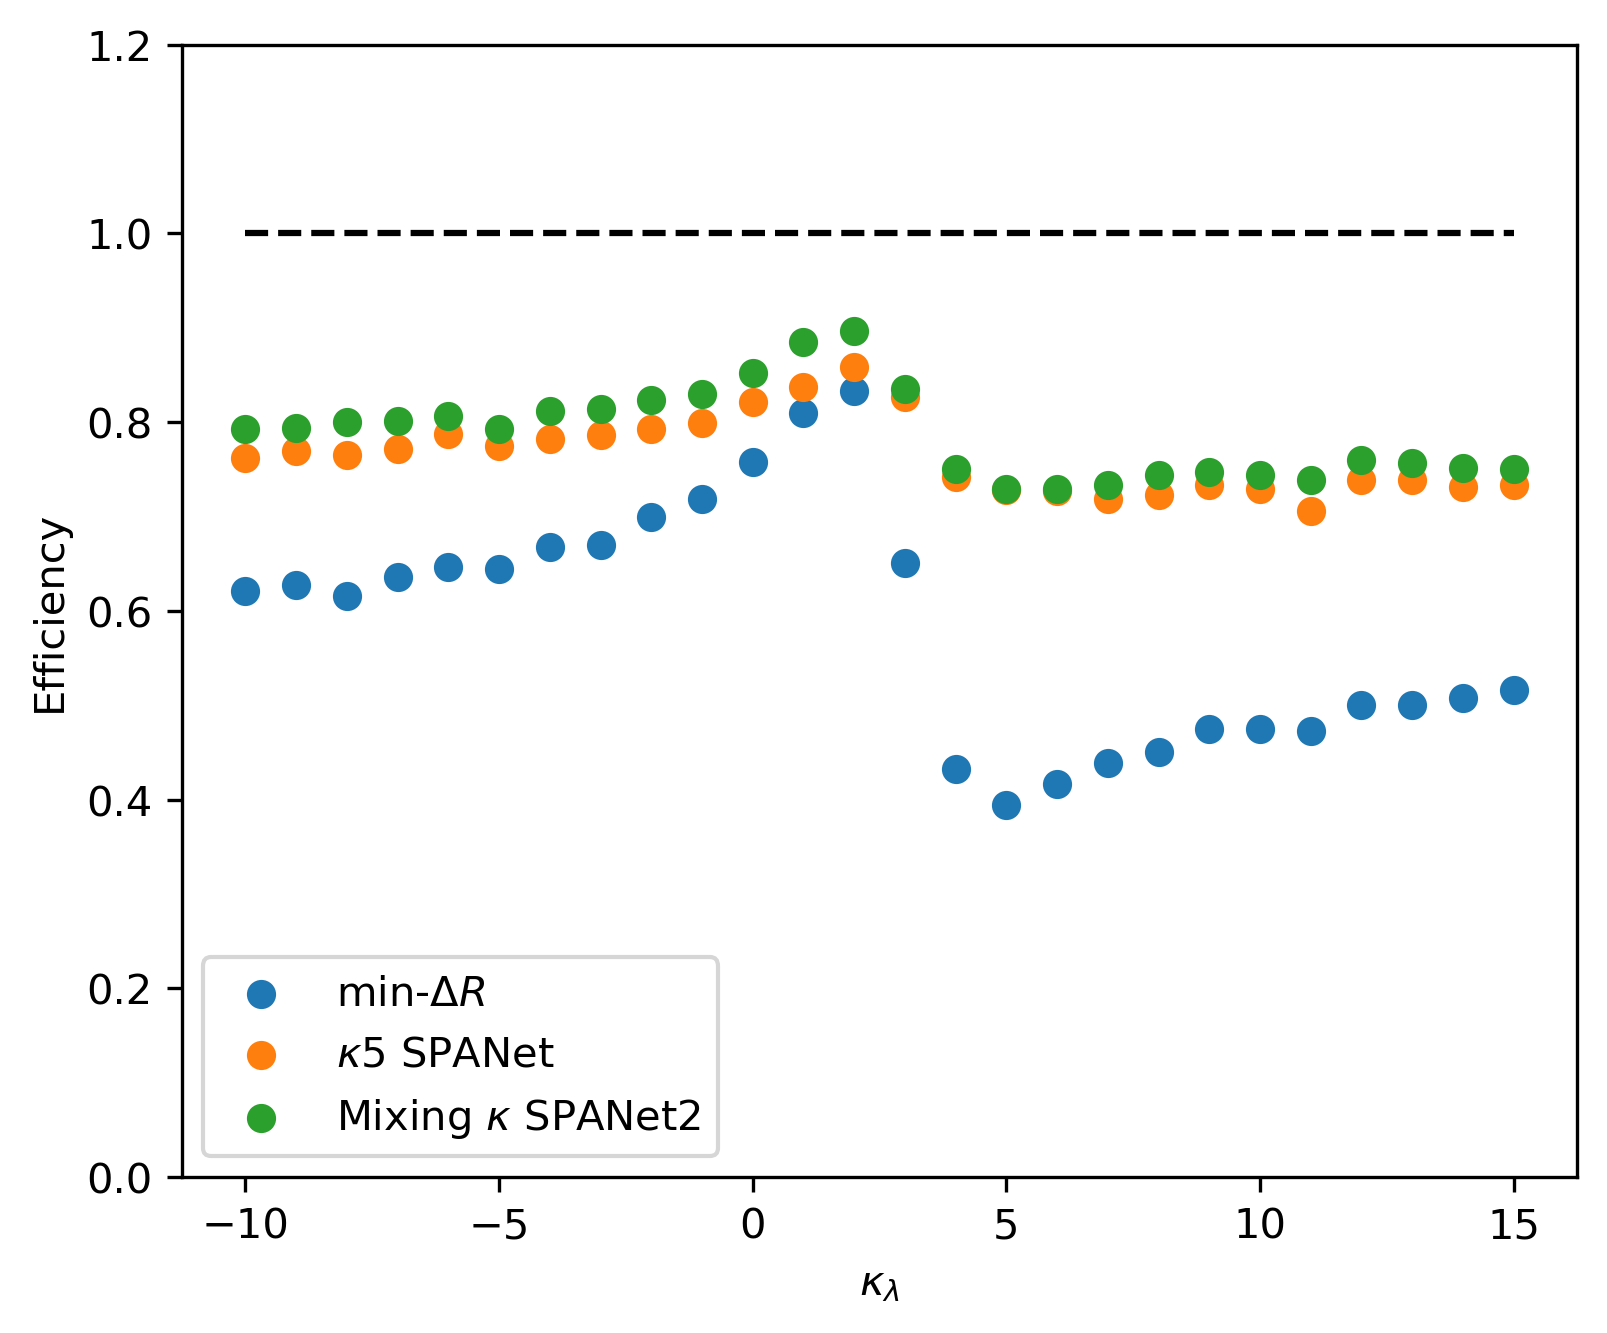
\includegraphics[width=0.65\textwidth]{pairing_efficiency_kappa-SPANet2.png}
			\caption{The pairing performance for different $\kappa_\lambda$ samples.}
			\label{fig:pairing_performance_kappa}
		\end{figure}

	% subsection pairing_performance (end)
	\subsection{Classification performance}% (fold)
	\label{sub:classification_performance}
		Table \ref{tab:SPANET_cls_results} presents the classification training results.
		\begin{table}[htpb]
			\centering
			\caption{The classification performance of different selection methods.}
			\label{tab:classification_results_summary}
			\begin{tabular}{c|cc}
			Selection method          & ACC   & AUC   \\ \hline
			$\text{min-}\Delta R$ DNN & 0.783 & 0.864 \\
			$\kappa 5$ SPANet DNN     & 0.792 & 0.875 \\
			mixing $\kappa$ SPANet2   & 0.828 & 0.911
			\end{tabular}			
		\end{table}

	% subsection classification_performance (end)
	\subsection{\texorpdfstring{$\kappa_\lambda$}{kappa} constraints}% (fold)
	\label{sub:kappa_constraints}
		Table \ref{tab:kappa_constraint_summary} is the $\kappa_\lambda$ constraints of the different selection methods.
		\begin{table}[htpb]
			\centering
			\caption{The $\kappa_\lambda$ constraints of different selection methods.}
			\label{tab:kappa_constraint_summary}
			\begin{tabular}{cc|cc|cc}
									&                  & \multicolumn{4}{c}{Expected Constraints}                         \\
									&                  & \multicolumn{2}{c}{Profile likelihood} & \multicolumn{2}{c}{CLs} \\ \hline
			Pairing method          & Selection method & Lower              & Upper             & Lower       & Upper     \\ \hline
			$\text{min-}\Delta R$   & DNN              & $-3.81$            & $11.16$           & $-3.73$     & $11.15$   \\
			$\kappa 5$ SPANet       & DNN              & $-4.08$            & $11.65$           & $-4.02$     & $11.68$   \\
			Mixing $\kappa$ SPANet2 & SPANet2          & $-3.48$            & $9.18$            & $-3.41$     & $9.09$   
			\end{tabular}		
		\end{table}


	% subsection kappa_constraints (end)
	\subsection{Mass distribution plot}% (fold)
	\label{sub:mass_distribution_plot}
		Figure \ref{fig:Higgs_mass_signal} and \ref{fig:Higgs_mass_background} show the Higgs mass distribution for signal and background events with different pairing methods. The selection does not apply. The mass planes for the signal process all look similar for all pairing methods. For background, the results of $\text{min-}\Delta R$ are very different from others.
		\begin{figure}[htpb]
			\centering
			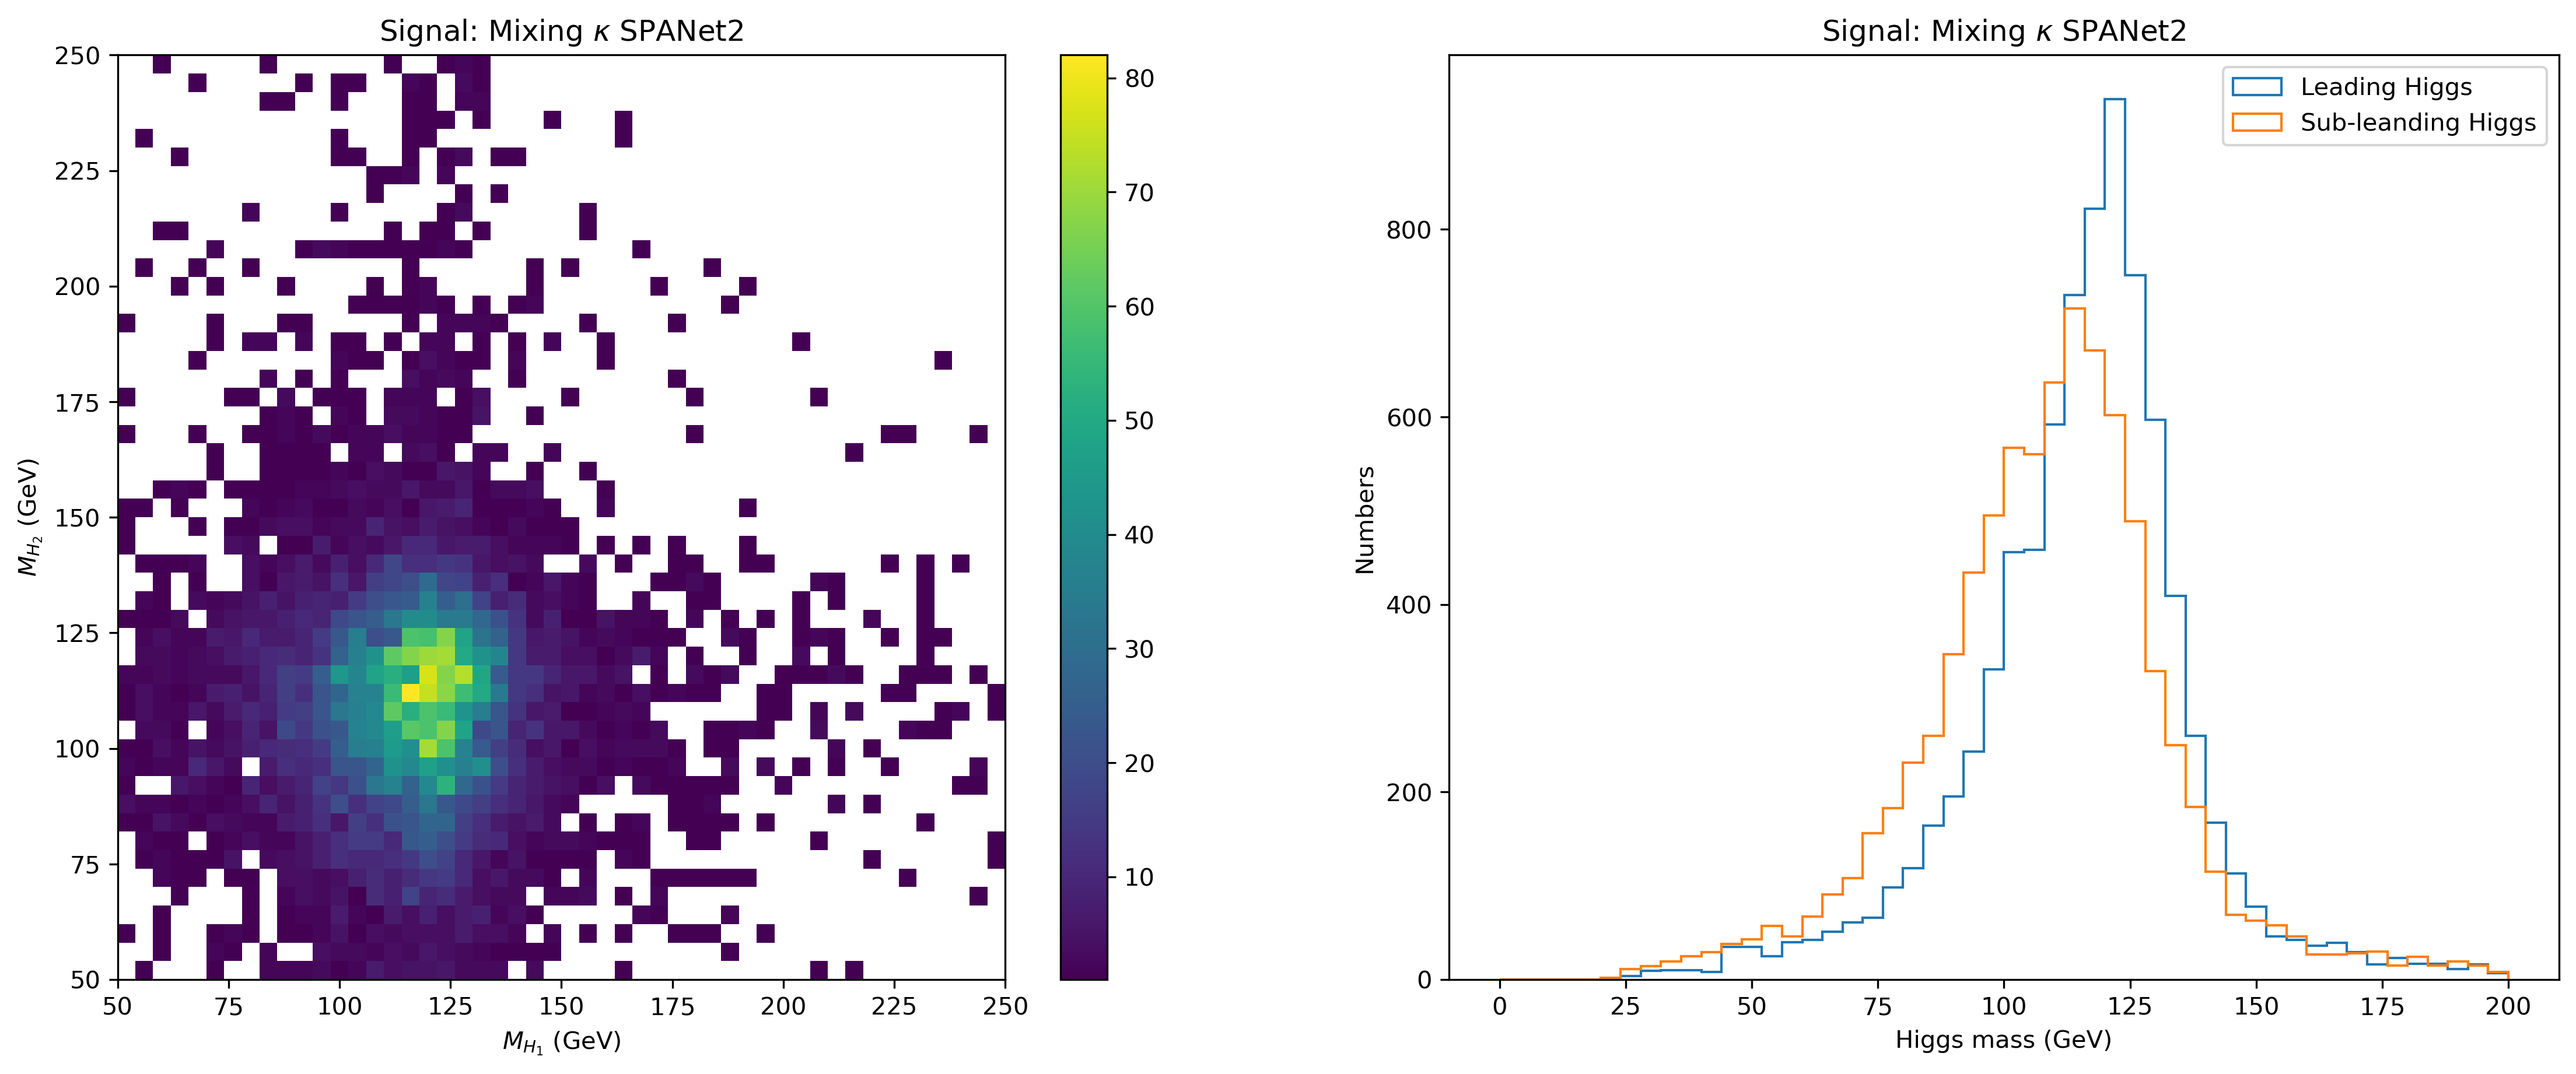
\includegraphics[width=0.97\textwidth]{Higgs_mass_mix-SPANET2_s.png}
			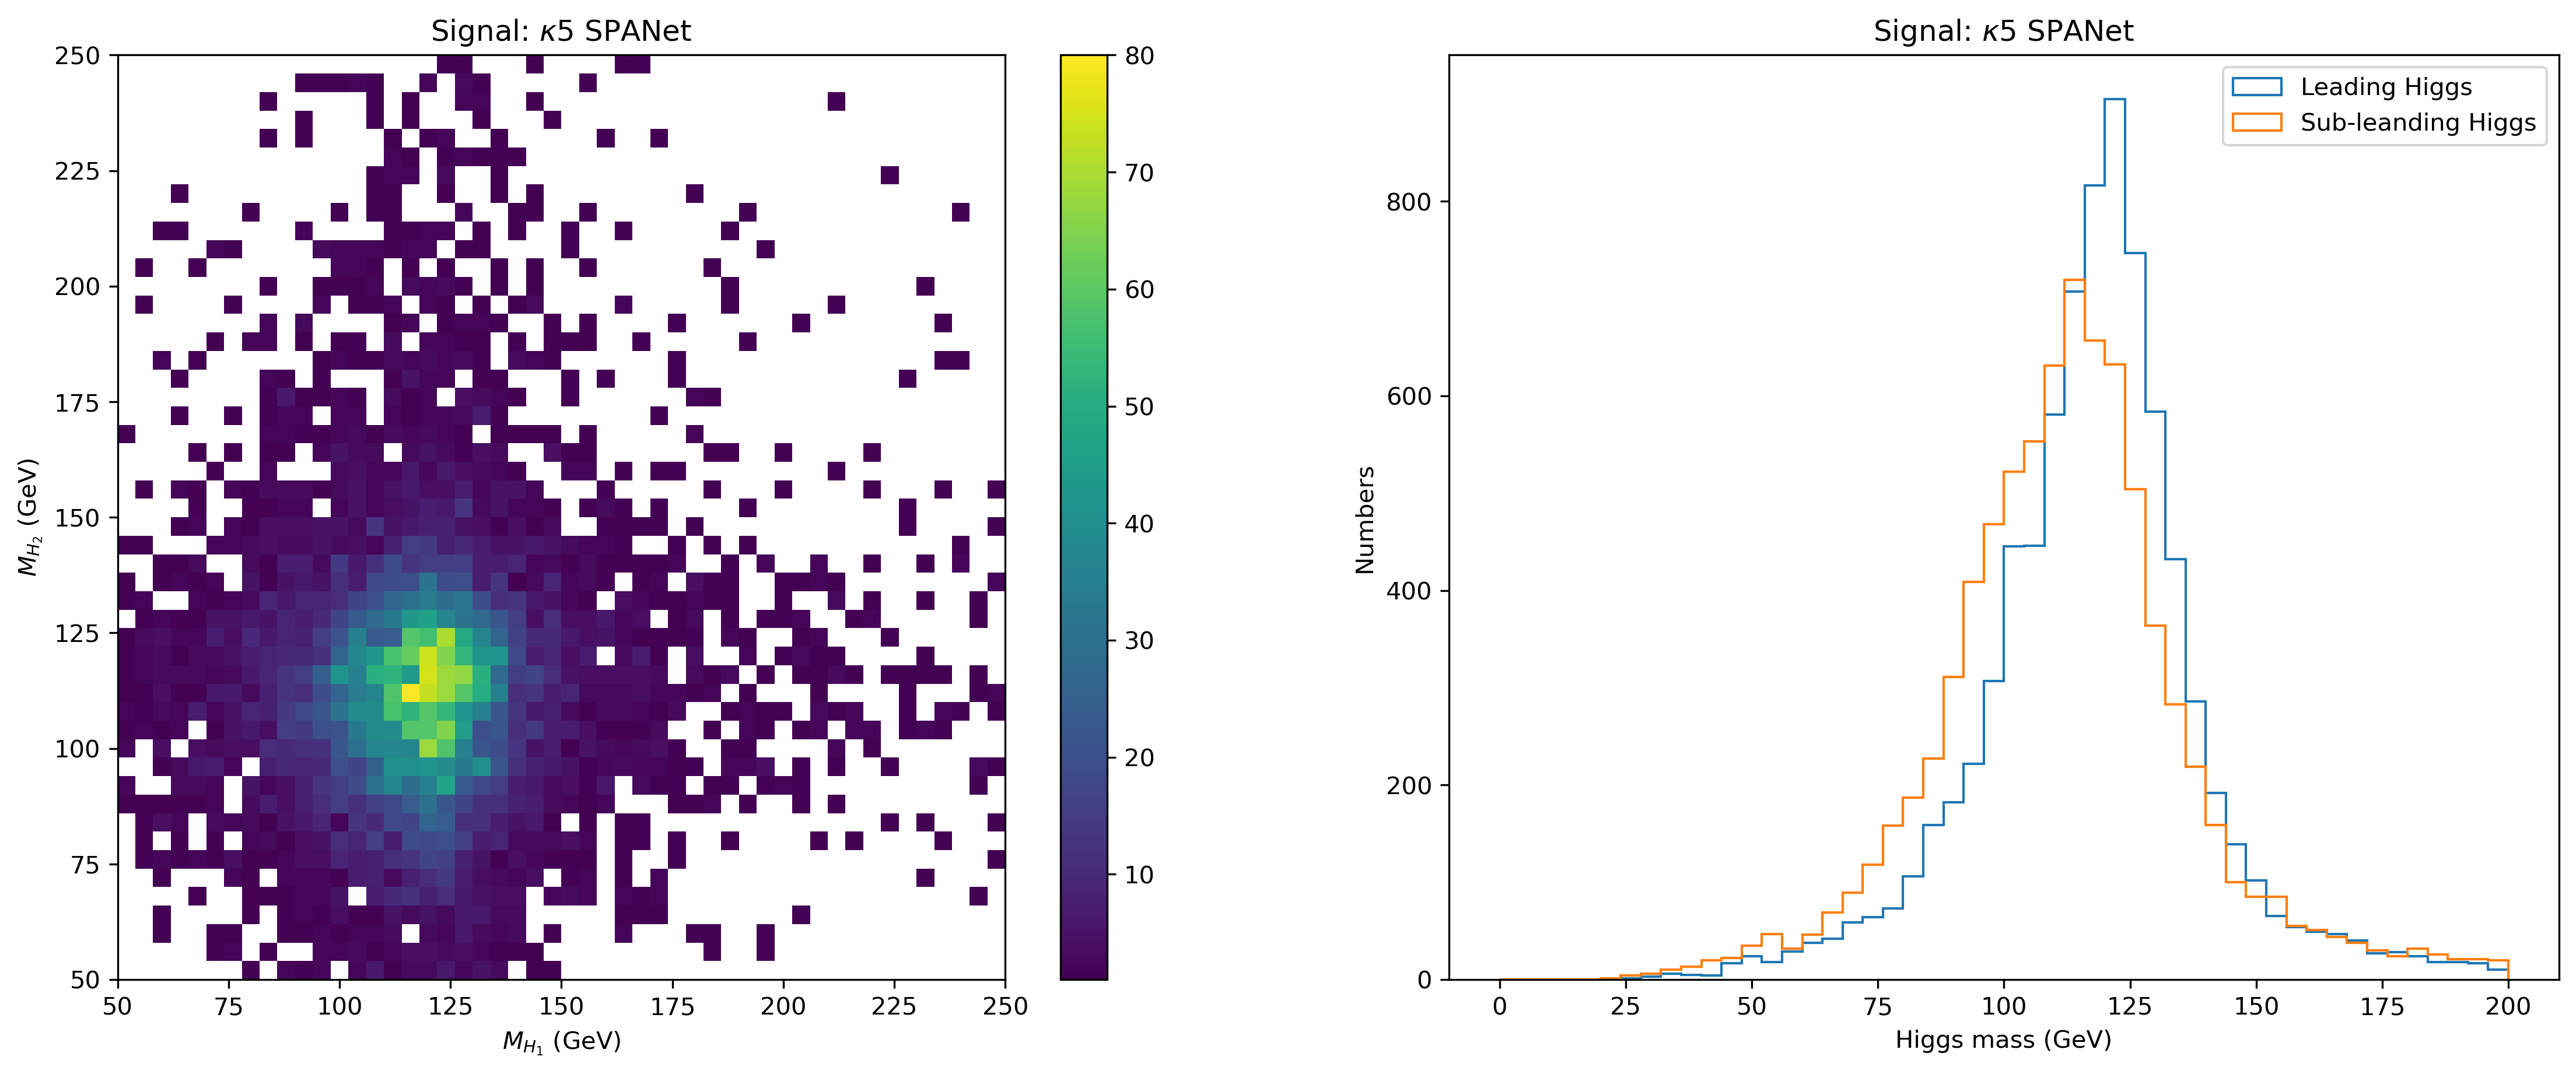
\includegraphics[width=0.97\textwidth]{Higgs_mass_k5-SPANET_s.png}
			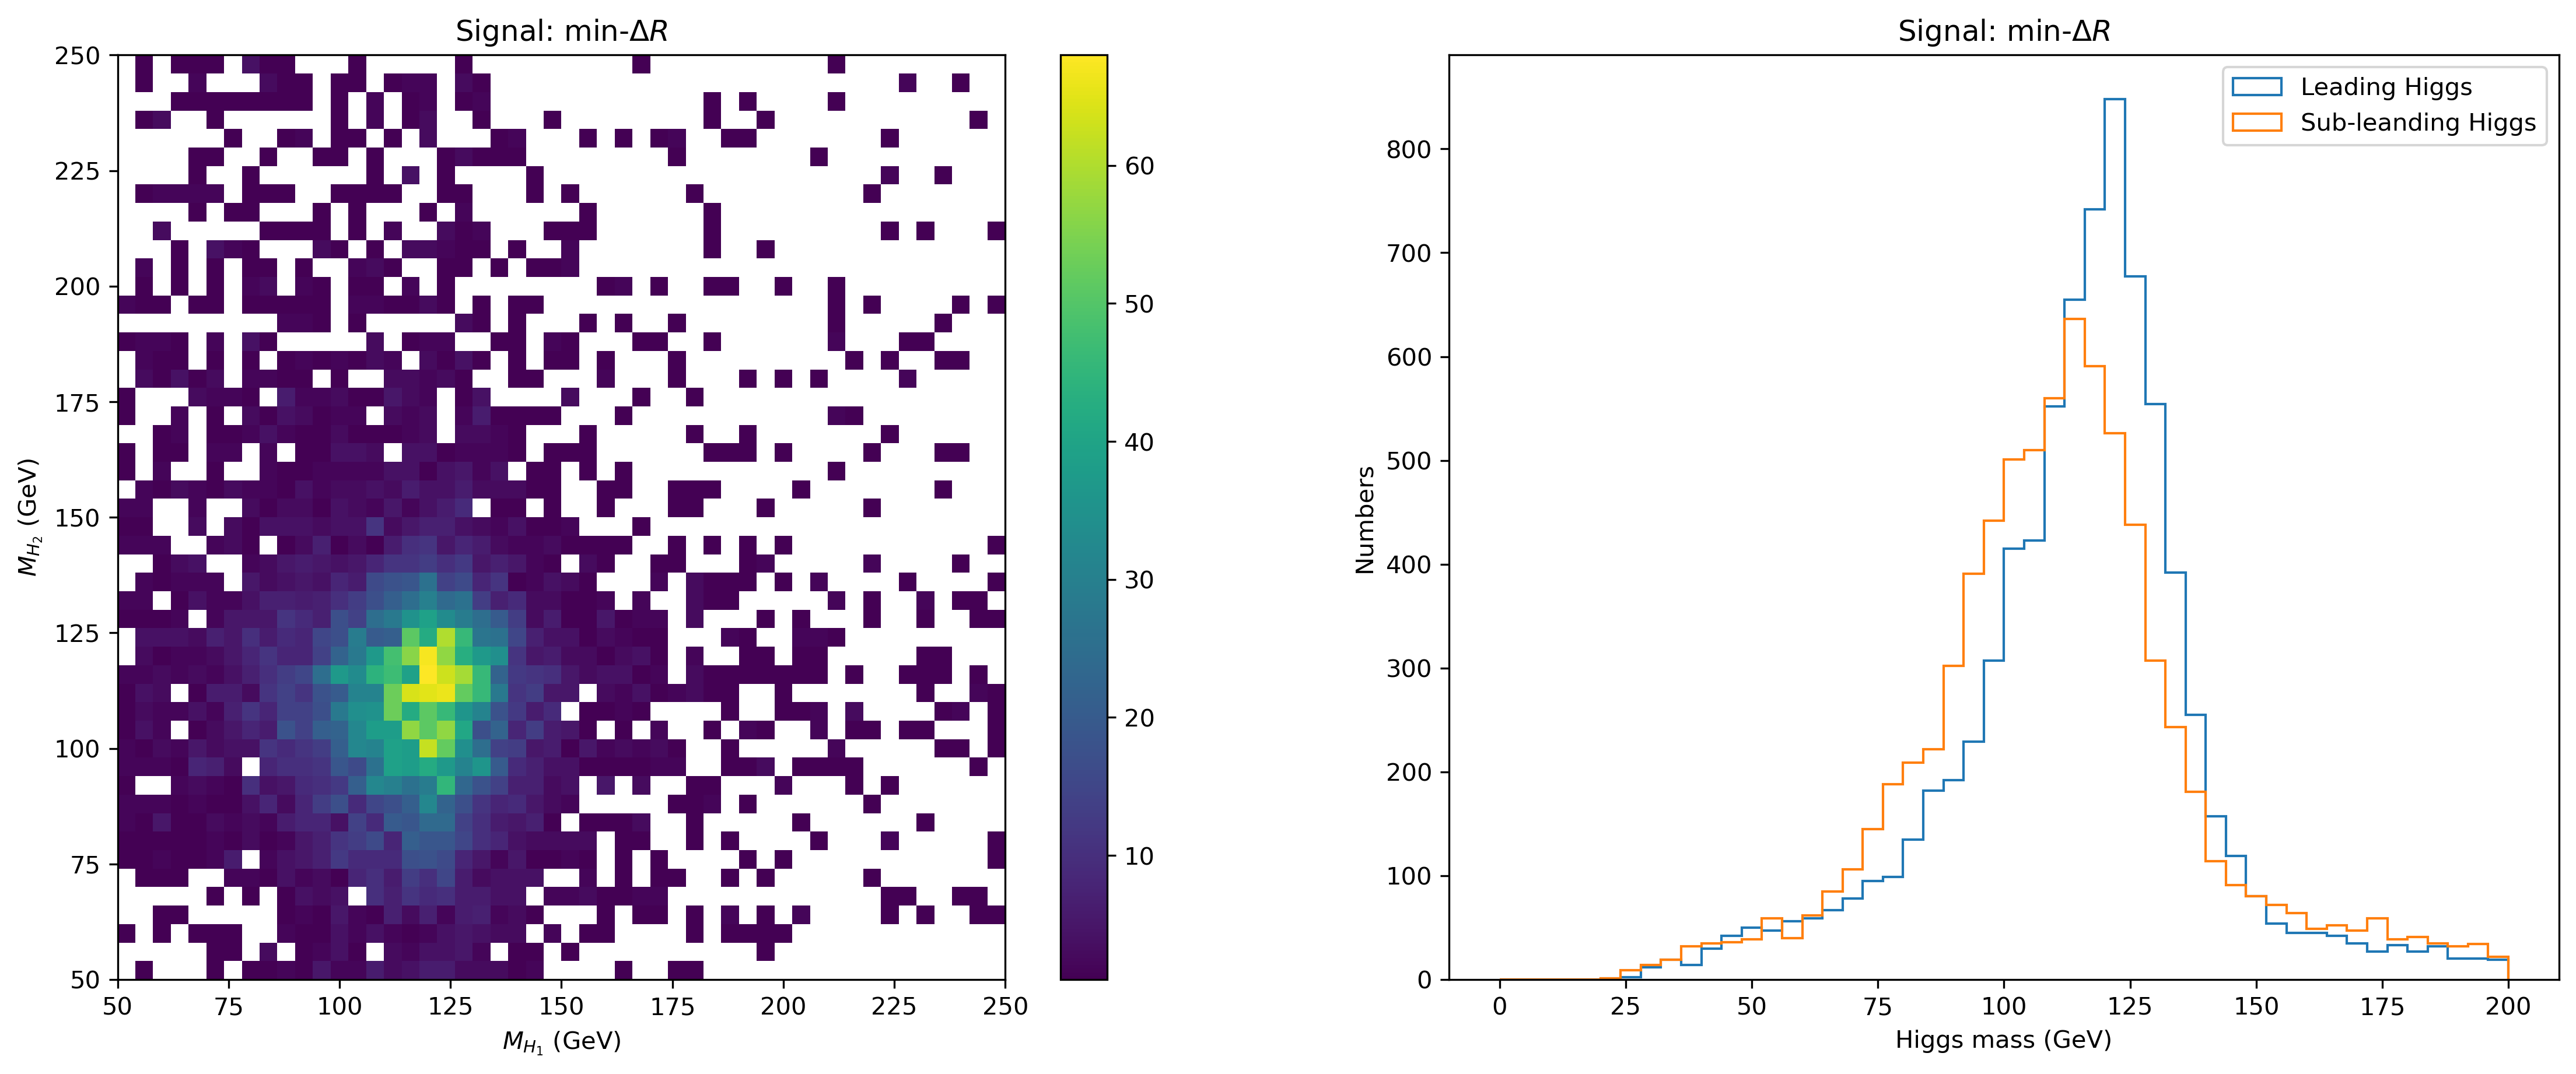
\includegraphics[width=0.97\textwidth]{Higgs_mass_mindR_s.png}
			\caption{The mass plane and distribution of Higgs candidate for signal events with different pairing methods. The top one is mixing $\kappa$ SPANet2 pairing, the middle one is $\kappa 5$ SPANet pairing, bottom one is $\text{min-}\Delta R$ pairing.}
			\label{fig:Higgs_mass_signal}
		\end{figure}

		\begin{figure}[htpb]
			\centering
			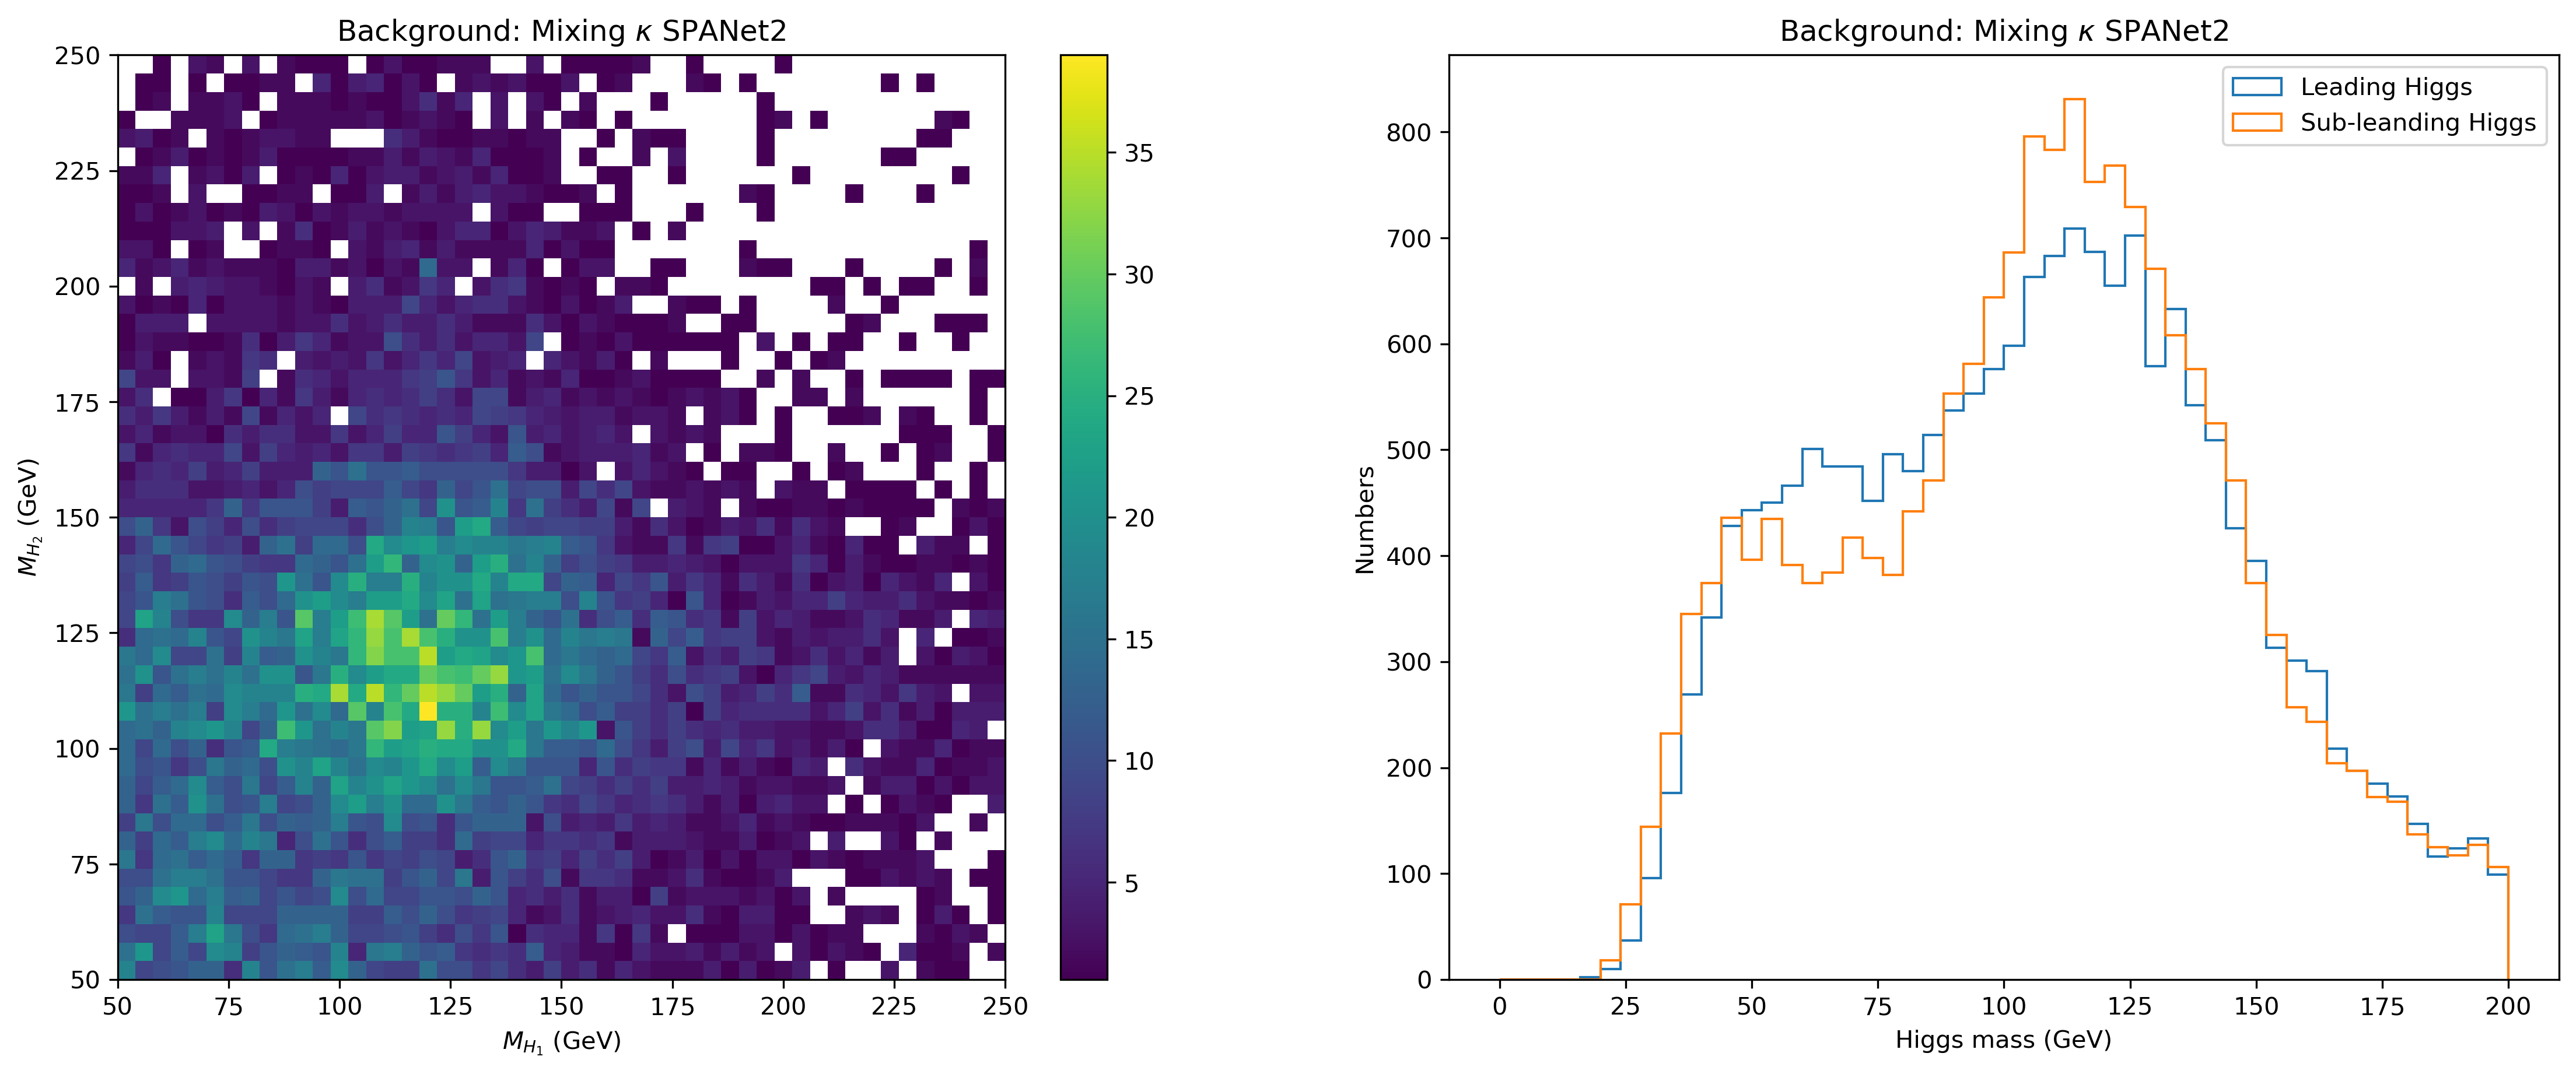
\includegraphics[width=0.97\textwidth]{Higgs_mass_mix-SPANET2_b.png}
			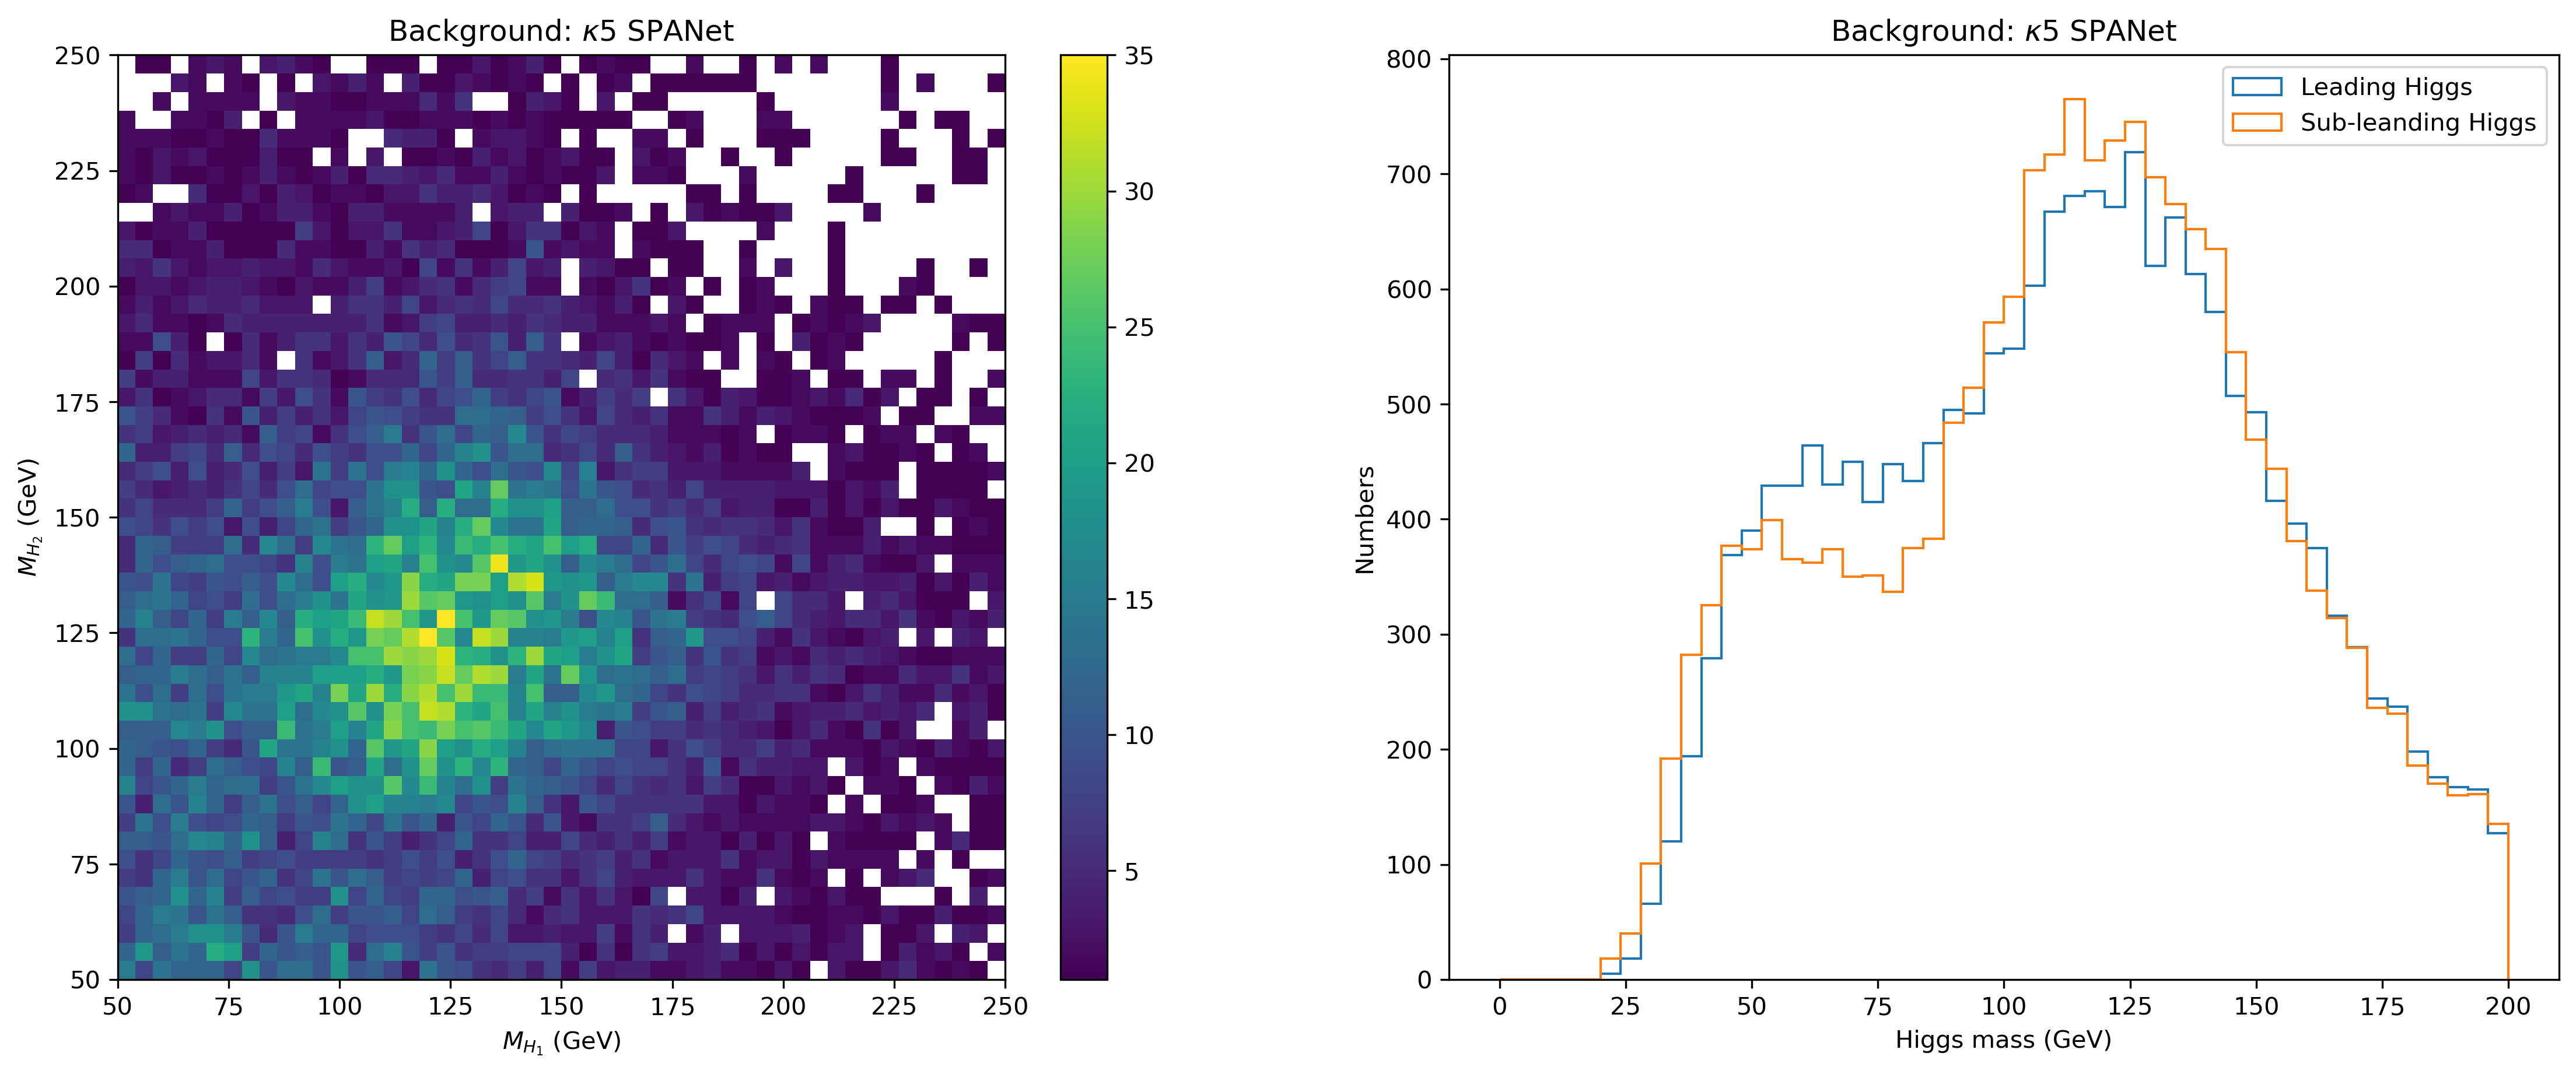
\includegraphics[width=0.97\textwidth]{Higgs_mass_k5-SPANET_b.png}
			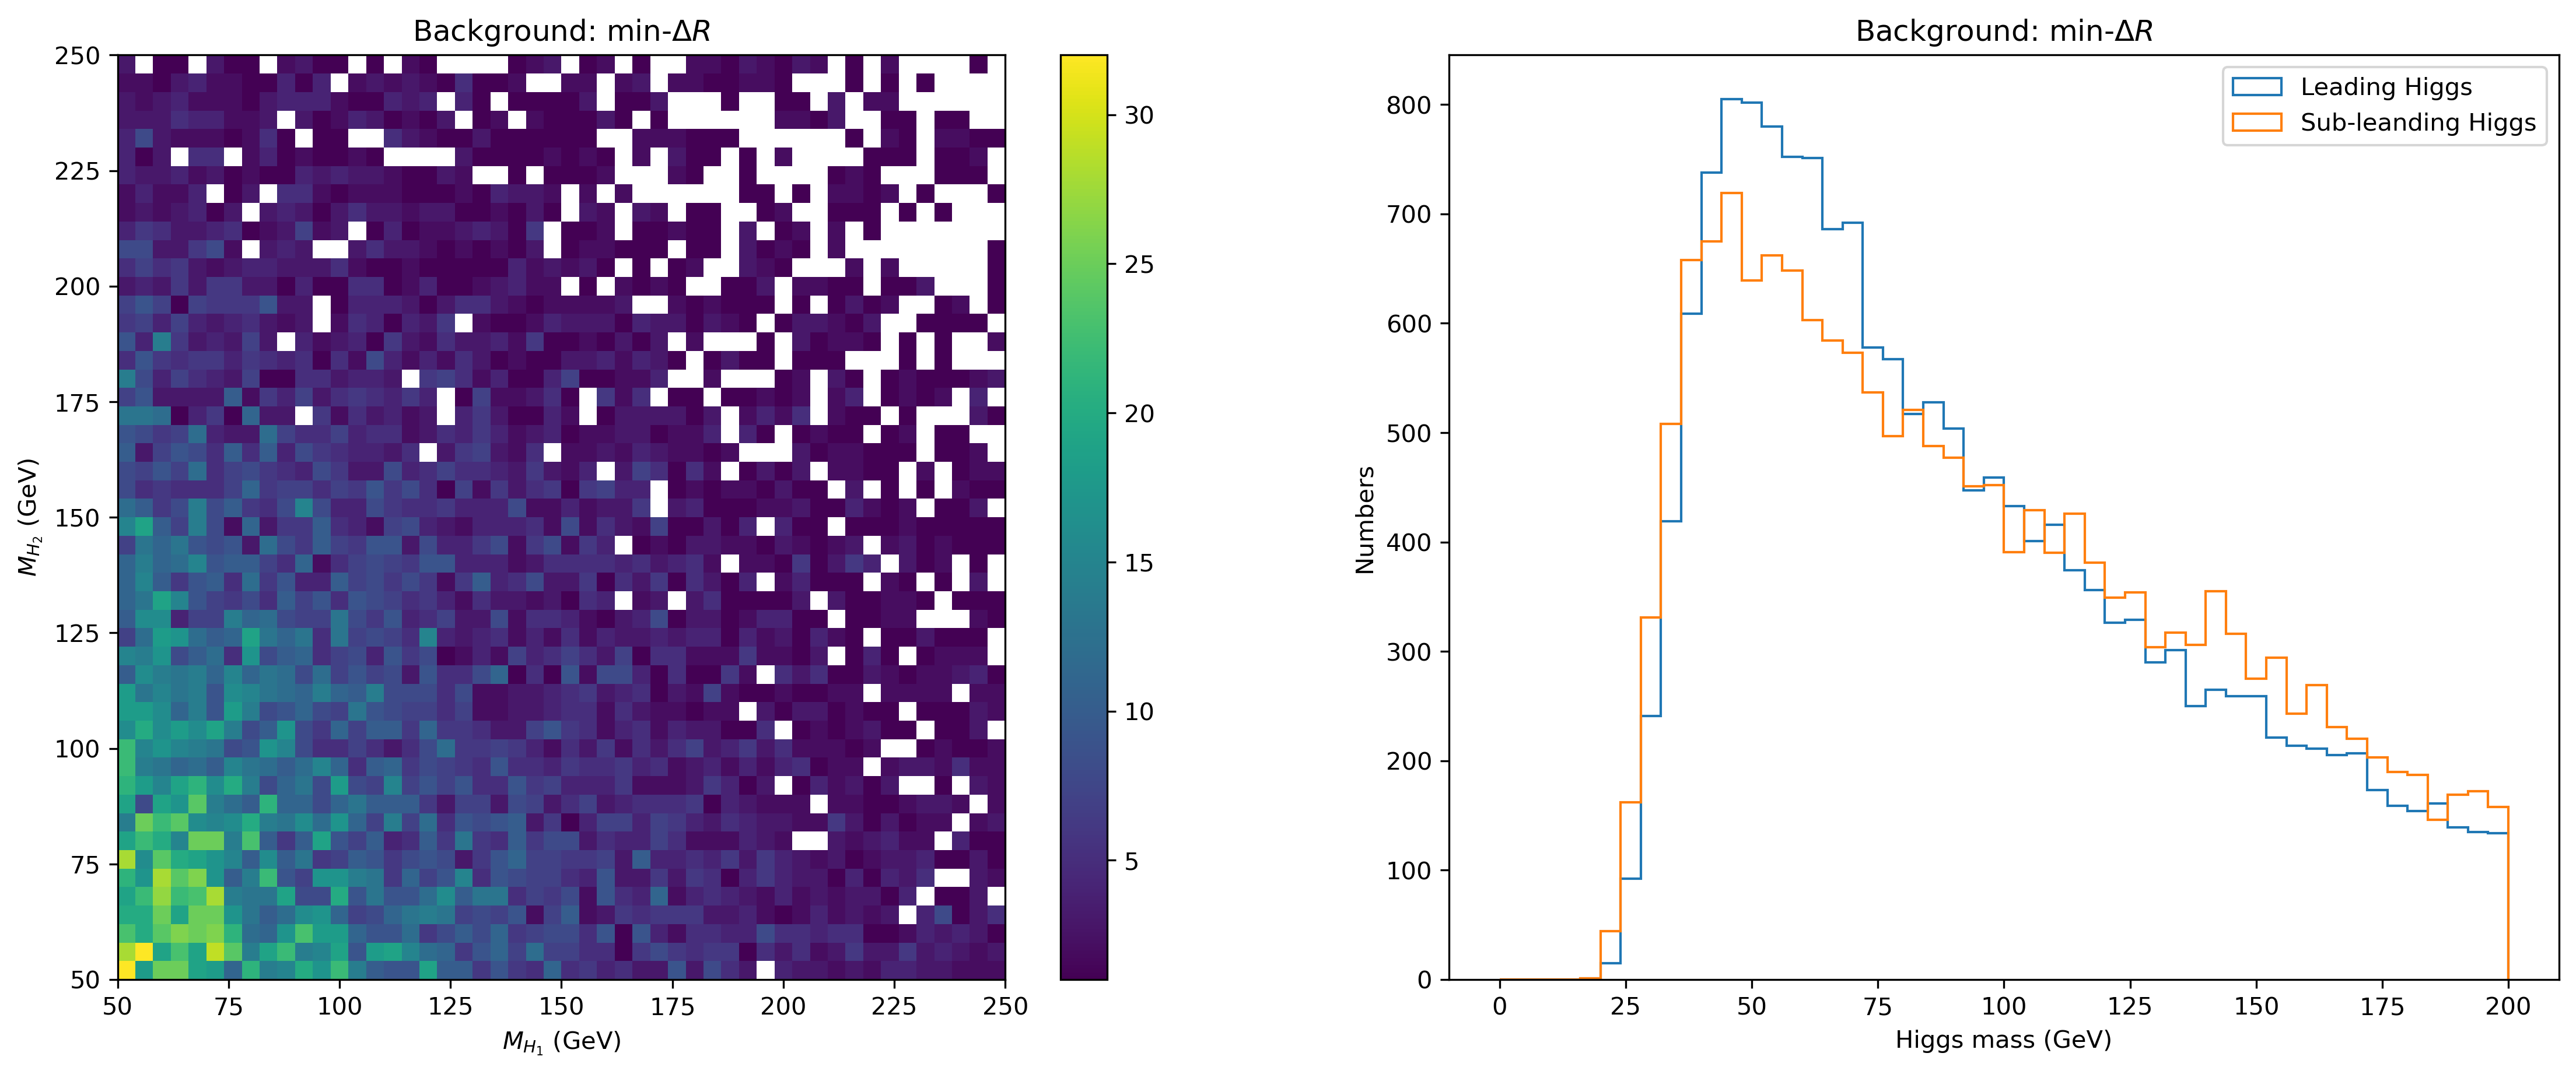
\includegraphics[width=0.97\textwidth]{Higgs_mass_mindR_b.png}
			\caption{The mass plane and distribution of Higgs candidate for background events with different pairing methods. The top one is mixing $\kappa$ SPANet2 pairing, the middle one is $\kappa 5$ SPANet pairing, bottom one is $\text{min-}\Delta R$ pairing.}
			\label{fig:Higgs_mass_background}
		\end{figure}


		Figure \ref{fig:mhh_distributions} are the $m_{HH}$ distributions after the selection.
		\begin{figure}[htpb]
			\centering
			\subfloat[$\text{min-}\Delta R$ DNN]{
				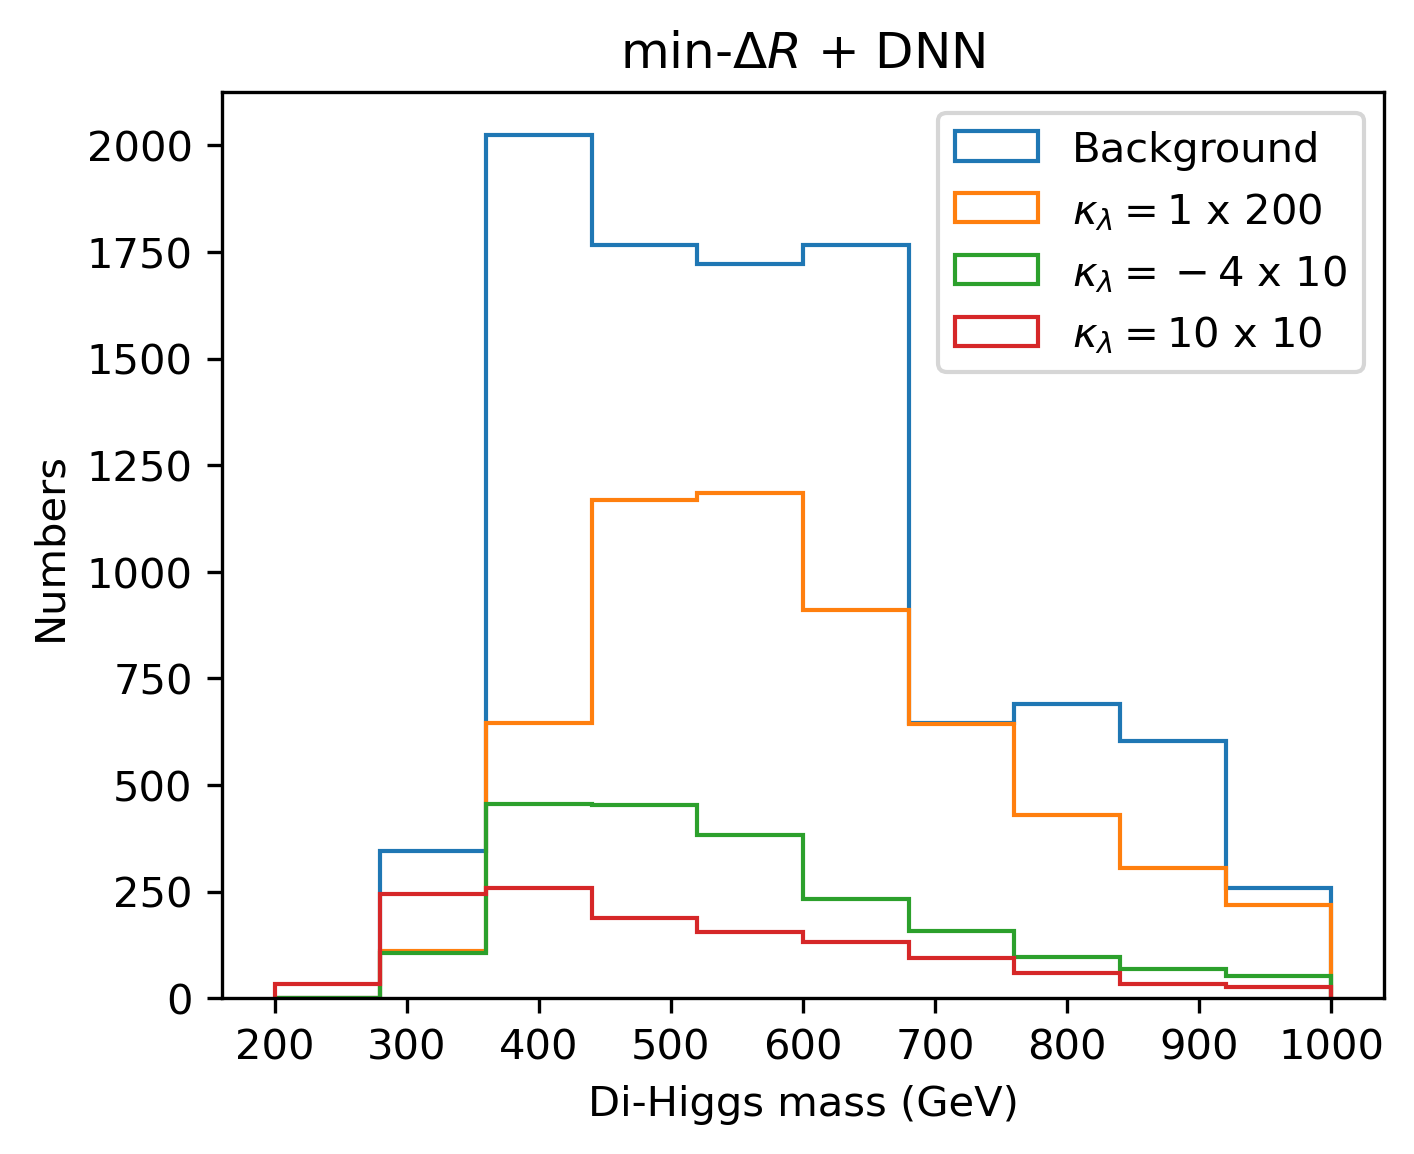
\includegraphics[width=0.30\textwidth]{mhh_DNN_min_dR.png}
			}
			\subfloat[$\kappa 5$ SPANet DNN]{
				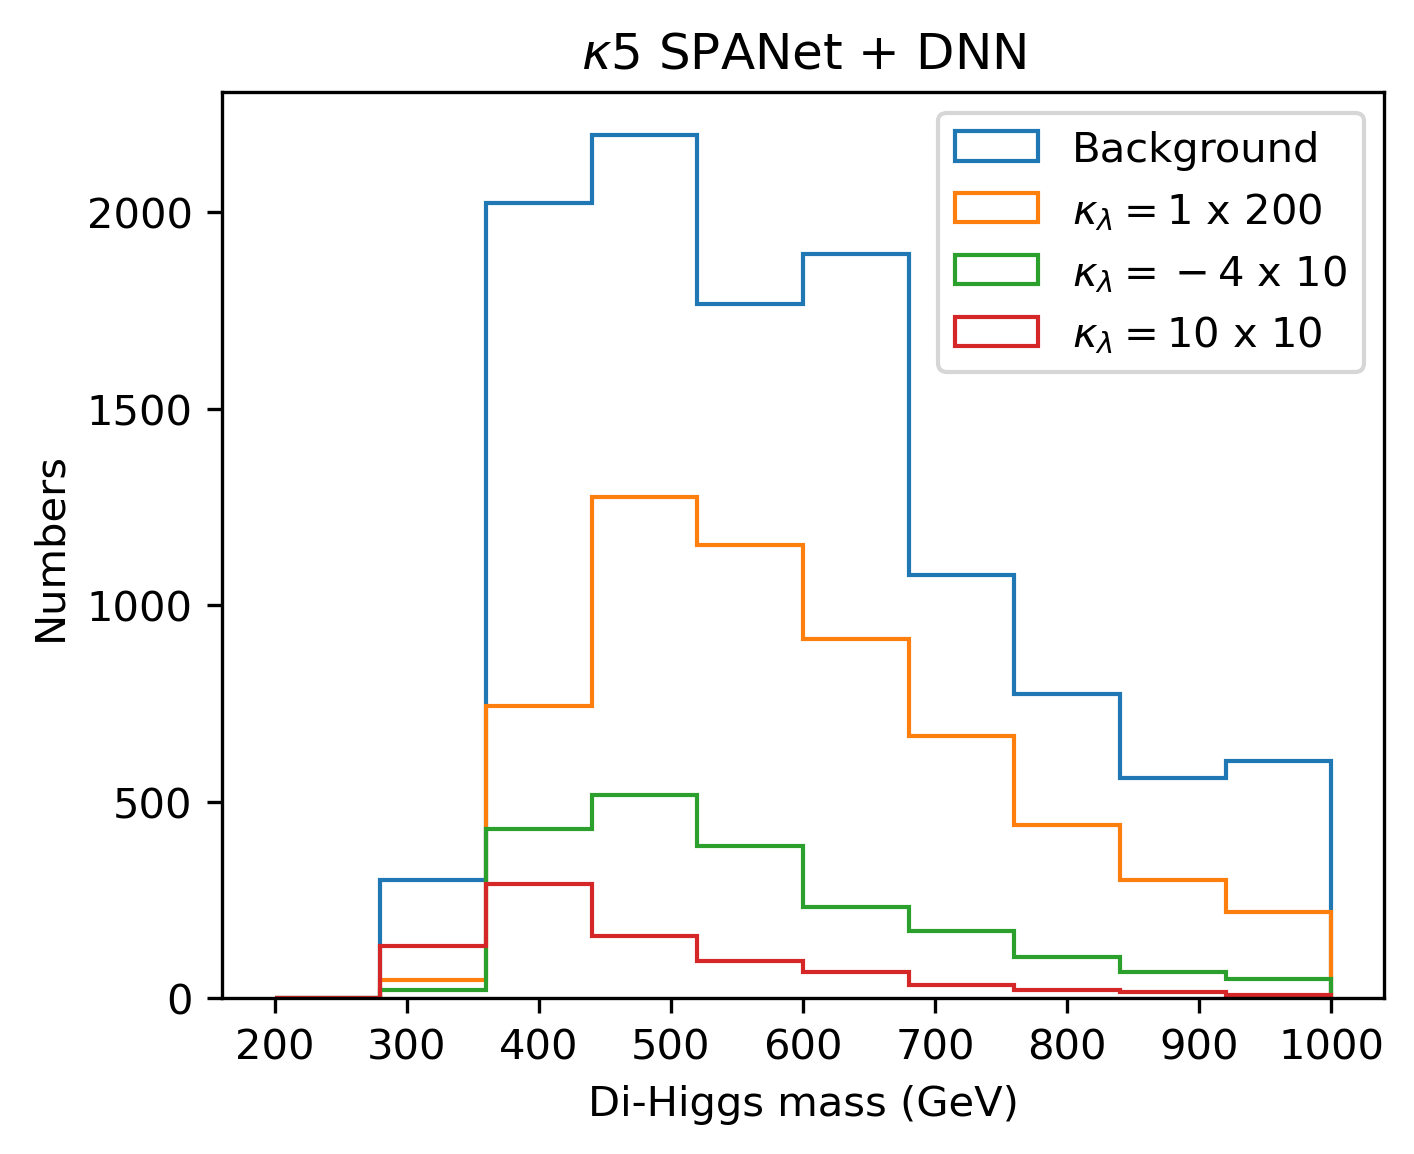
\includegraphics[width=0.30\textwidth]{mhh_DNN_k5_SPANET.png}
			}
			\subfloat[Mixing $\kappa$ SPANet2]{
				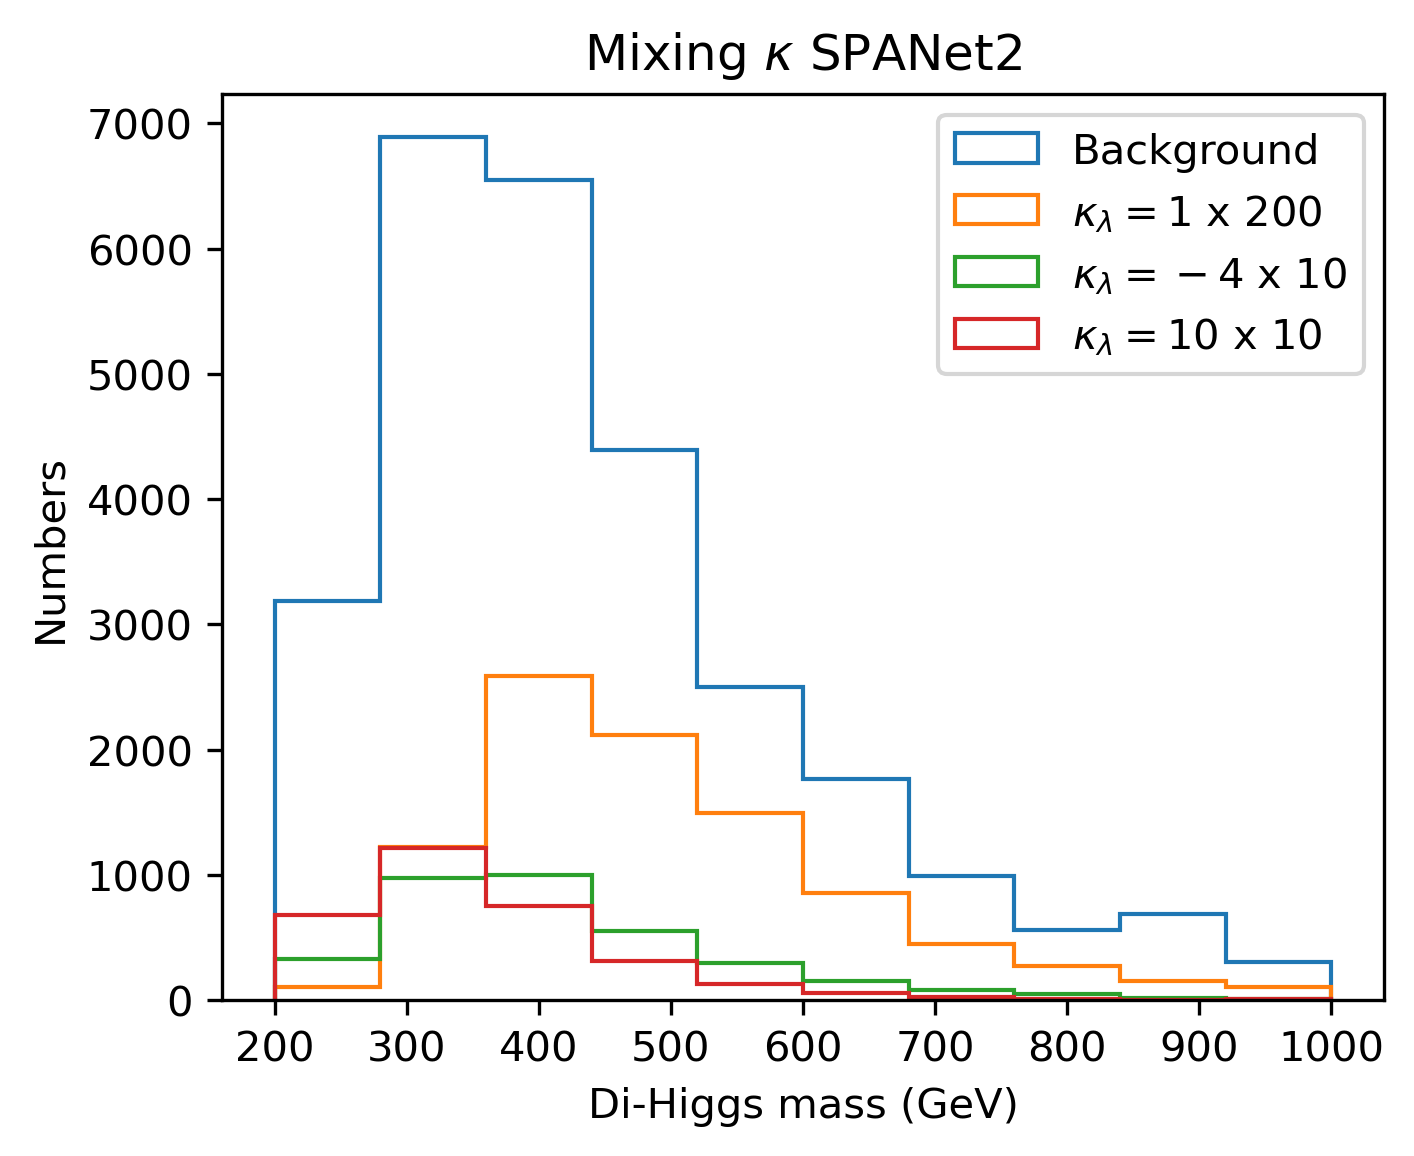
\includegraphics[width=0.30\textwidth]{mhh_mix_SPANET2.png}
			}
			\caption{The $m_{H H}$ distributions after selection. The DNNs are trained with different pairing method samples.}
			\label{fig:mhh_distributions}
		\end{figure}
		
	% subsection mass_distribution_plot (end)
% section comparision_with_previous_results (end)		
\section{SPANet2 pairing + DNN selection}% (fold)
\label{sec:spanet2_pairing_dnn_selection}
	This section uses the mixing $\kappa$ SPANet2 for jet pairing and generates the samples for DNN training. The training samples consisted of different $\kappa_\lambda$ value events.

	\subsection{Training samples}% (fold)
	\label{sub:training_samples2}
	Set $\kappa_\lambda = [-5, -3, -1, 1, 2, 3, 5, 7, 9, 11]$, for each $\kappa_\lambda$ point generate samples. For signal, the different $\kappa_\lambda$ samples are mixed. For each type, the same number of samples is used. For background, the $\kappa_\lambda$ values are randomly chosen from the above list. Training sample sizes are shown in Table \ref{tab:DNN_sample_size3}.
		\begin{table}[htpb]
			\centering
			\caption{The sample size for signal and background, which are the training and testing sample sizes.}
			\label{tab:DNN_sample_size3}
			\begin{tabular}{c|c}
			 Signal & Background\\ \hline
			 $\text{80k} + \text{8k}$      &$\text{80k} + \text{8k}$ 
			\end{tabular}
		\end{table}

	% subsection training_samples (end)
	\subsection{Training results}% (fold)
	\label{sub:training_results}
		The DNN training results are summarized in Table \ref{tab:DNN_results}.
		\begin{table}[htpb]
			\centering
			\caption{The DNN training results with different pairing methods. The training samples contain different $\kappa_\lambda$ samples. The average and standard deviation of 10 training is presented.}
			\label{tab:DNN_results}
			\begin{tabular}{c|cc}
			Pairing method        & ACC     & AUC   \\ \hline
			$\text{min-}\Delta R$ & $0.800 \pm 0.010$ & $0.882 \pm 0.010$ \\
			$\kappa 5$ SPA-NET    & $0.794 \pm 0.004$ & $0.876 \pm 0.004$ \\
			mixing $\kappa$ SPANet2 & $0.800 \pm 0.003$ & $0.882 \pm 0.004$ \\
			\end{tabular}      
		\end{table}
	
	% subsection training_results (end)
	\subsection{\texorpdfstring{$\kappa_\lambda$}{kappa} limits}% (fold)
	\label{sub:kappa_limits}
		Set the $\kappa_\lambda$ limits by the profile likelihood method and CLs method. The model with the best ACC is used. The $p_\text{th}$ is chosen such that maximize $S / \sqrt{B}$.

		The results of $\kappa_\lambda$ constraints are summarized in Table \ref{tab:kappa_constraint_DNN}. 
		\begin{table}[htpb]
			\centering
			\caption{The $\kappa_\lambda$ constraints with DNN selection samples.}
			\label{tab:kappa_constraint_DNN}
			\begin{tabular}{c|cc|cc}
								  & \multicolumn{4}{c}{Expected Constraint}                          \\
								  & \multicolumn{2}{c}{Profile likelihood} & \multicolumn{2}{c}{CLs} \\ \hline
			Pairing method        & Lower              & Upper             & Lower      & Upper      \\ \hline
			$\text{min-}\Delta R$ & $-3.20$            & $10.87$             & $-3.16$      & $10.78$    \\
			$\kappa 5$ SPA-NET    & $-4.44$            & $10.86$             & $-4.35$      & $10.78$   \\
			mixing $\kappa$ SPANet2& $-3.42$           & $10.85$             & $-3.40$      & $10.77$   
			\end{tabular}
		\end{table}

		Here, the bug of the previous testing sample is fixed. In the previous background testing sample, all $\kappa_\lambda$ are set to $1$ not randomly chosen from $\kappa_\lambda$ value list.
	% subsection kappa_limits (end)
% section spanet2_pairing_dnn_selection (end)
\section{Summary}% (fold)
\label{sec:summary}
	\subsection{Classification performance}% (fold)
	\label{sub:classification_performance}
		Table \ref{tab:classification_results_summary2} presents the classification training results.
		\begin{table}[htpb]
			\centering
			\caption{The classification performance of different selection methods.}
			\label{tab:classification_results_summary2}
			\begin{tabular}{l|cc}
			Selection method          & ACC   & AUC   \\ \hline
			$\text{min-}\Delta R$ DNN   & $0.800 \pm 0.010$ & $0.882 \pm 0.010$ \\
			$\kappa 5$ SPANet DNN       & $0.794 \pm 0.004$ & $0.876 \pm 0.004$ \\
			mixing $\kappa$ SPANet2 DNN & $0.800 \pm 0.003$ & $0.882 \pm 0.004$ \\
			mixing $\kappa$ SPANet2     & $0.822 \pm 0.007$ & $0.906 \pm 0.006$ 
			\end{tabular}			
		\end{table}

	% subsection classification_performance (end)
	\subsection{\texorpdfstring{$\kappa_\lambda$}{kappa} constraints}% (fold)
	\label{sub:kappa_constraints}
		Table \ref{tab:kappa_constraint_summary2} is the $\kappa_\lambda$ constraints of the different selection methods.
		\begin{table}[htpb]
			\centering
			\caption{The $\kappa_\lambda$ constraints of different selection methods.}
			\label{tab:kappa_constraint_summary2}
			\begin{tabular}{cc|cc|cc}
									&                  & \multicolumn{4}{c}{Expected Constraints}                         \\
									&                  & \multicolumn{2}{c}{Profile likelihood} & \multicolumn{2}{c}{CLs} \\ \hline
			Pairing method          & Selection method & Lower              & Upper             & Lower       & Upper     \\ \hline
			$\text{min-}\Delta R$   & DNN              & $-3.20$            & $10.87$           & $-3.16$      & $10.78$    \\
			$\kappa 5$ SPANet       & DNN              & $-4.44$            & $10.86$           & $-4.35$      & $10.78$   \\
			Mixing $\kappa$ SPANet2 & DNN              & $-3.42$            & $10.85$           & $-3.40$      & $10.77$   \\
			Mixing $\kappa$ SPANet2 & SPANet2          & $-3.18$            & $8.79$            & $-3.13$      & $8.77$   
			\end{tabular}		
		\end{table}
	% subsection kappa_constraints (end)
	
% section summary (end)		
\section{\texorpdfstring{$\kappa_\lambda$}{kappa} constraints with different luminosities}% (fold)
\label{sec:kappa_constraints_with_different_luminosities}
	Use the $\text{min-}\Delta R$ method to set constraints with different luminosity. The results are shown in Figure \ref{fig:kappa_constraint_luminosity}.
	\begin{figure}[htpb]
		\centering
		\subfloat[]{
			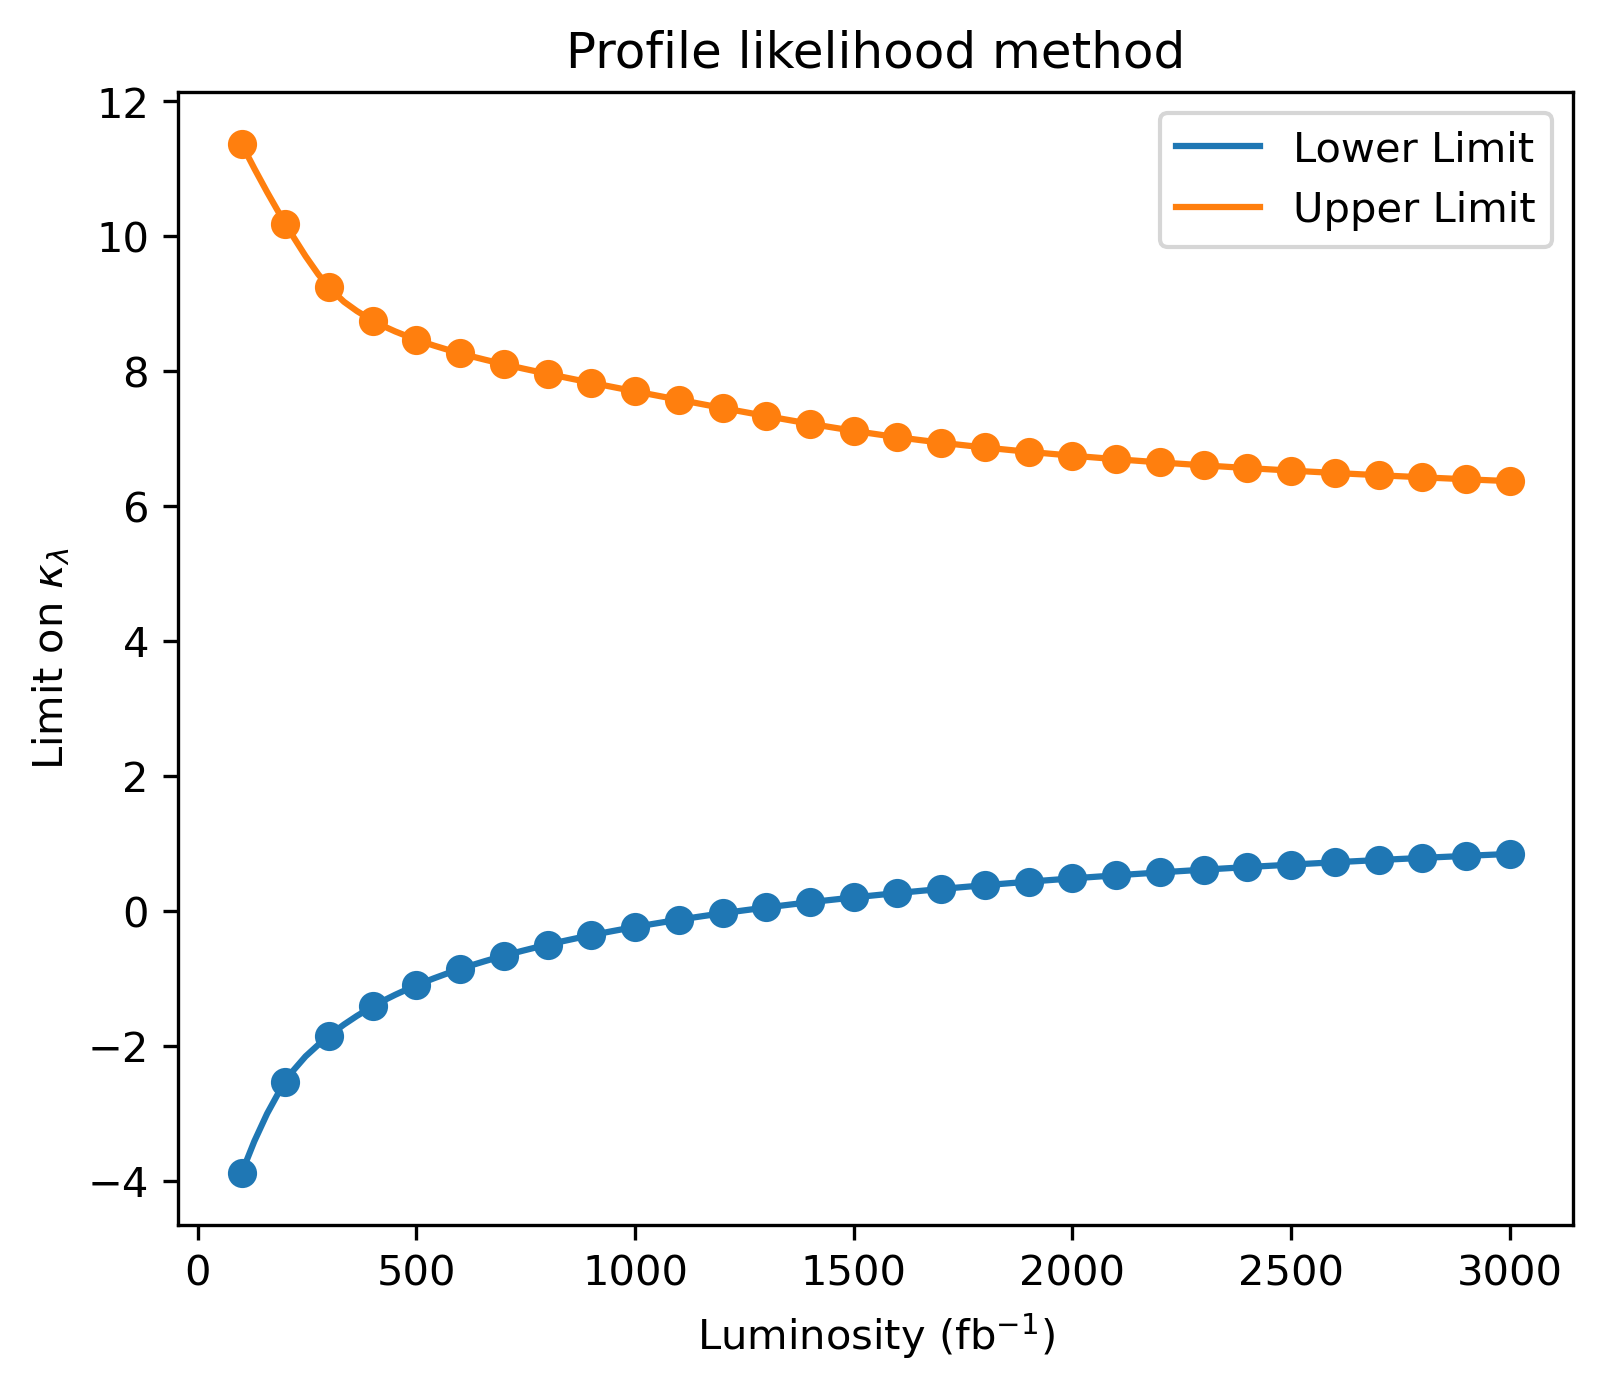
\includegraphics[width=0.45\textwidth]{kappa_constraint_LLr_L_mindR_DNN.png}
		}
		\subfloat[]{
			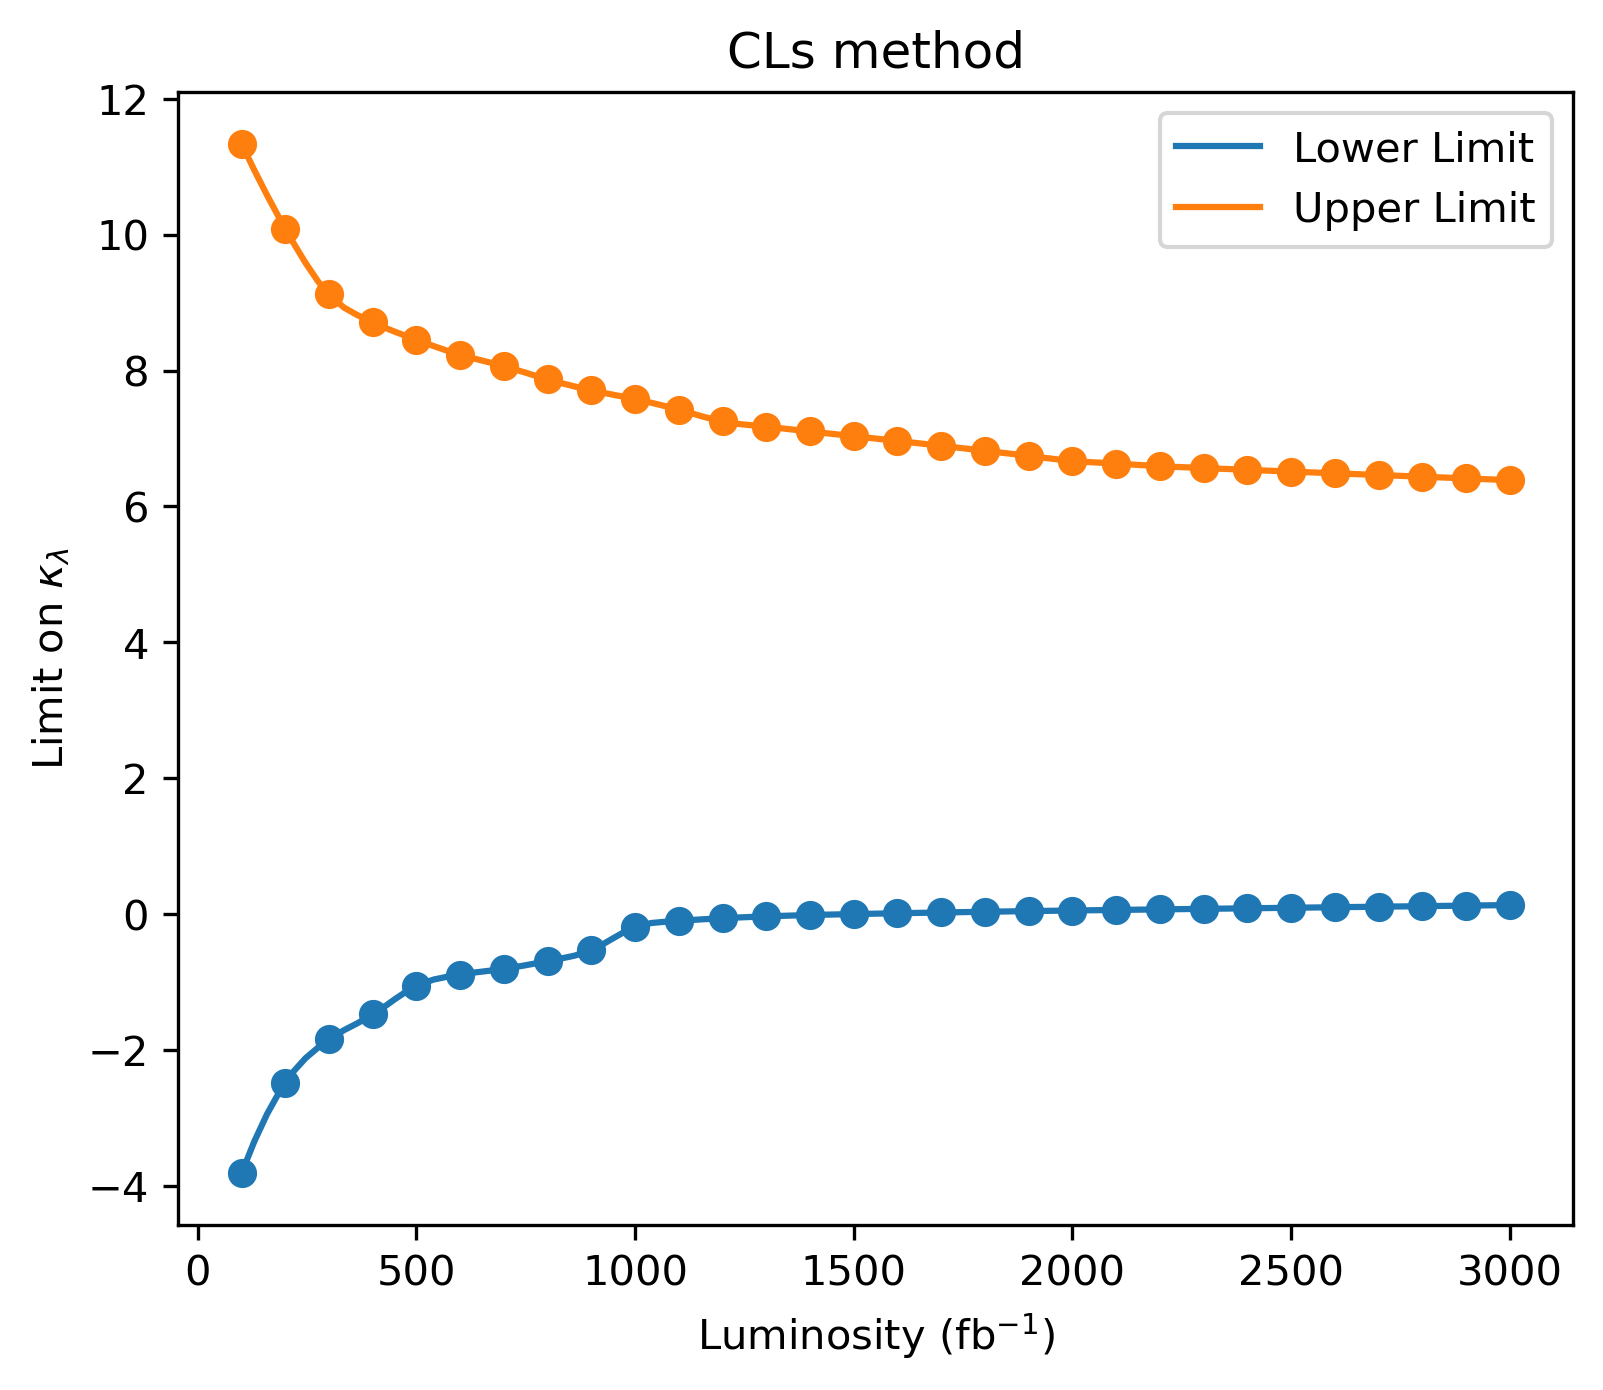
\includegraphics[width=0.45\textwidth]{kappa_constraint_CLs_L_mindR_DNN.png}
		}
		\caption{The $\kappa_\lambda$ constraints with different luminosities. Use $\text{min-}\Delta R$ method for pairing and DNN for selection.}
		\label{fig:kappa_constraint_luminosity}
	\end{figure}

	Use mixing $\kappa$ SPANet2 for constraints setting with different luminosity. The results are presented in Table \ref{tab:kappa_constraint_luminosity_mix_class_SPANET2}.
	\begin{table}[htpb]
		\centering
		\caption{The $\kappa_\lambda$ constraints with different luminosities. Use SPANet2 for event selection.}
		\label{tab:kappa_constraint_luminosity_mix_class_SPANET2}
		\begin{tabular}{c|cc|cc|cc|cc}
										& \multicolumn{4}{c}{Expected Constraints}                         & \multicolumn{4}{c}{Equivlent luminosity for $\text{min-}\Delta R$}       \\
										& \multicolumn{2}{c}{Profile likelihood} & \multicolumn{2}{c}{CLs} & \multicolumn{2}{c}{Profile likelihood} & \multicolumn{2}{c}{CLs}         \\ \hline
		$\mathcal{L} \text{ (fb$^{-1}$)}$ & Lower               & Upper            & Lower       & Upper     & Lower              & Upper             & Lower          & Upper          \\ \hline
		139  & $-3.18$ & $8.79$ & $-3.13$ & $8.77$ & 145 & 388 & 144 & 381 \\
		300  & $-1.96$ & $7.96$ & $-1.96$ & $7.89$ & 280 & 810 & 275 & 796 \\
		\end{tabular}
	\end{table}
% section kappa_constraints_with_different_luminosities (end)
\section{SPANet classifier}% (fold)
\label{sec:spanet_classifier}
	Figure \ref{fig:SPANet2_structure} is the model structure of SPANet2. The classifier part takes the outputs of the transformer encoder. The architecture of the classifier part is just the feed-forward structure networks.
	
	The SPANet classifier does not take the results from the jet assignment part, because it is worse than if we just take the transformer outputs. The reason is that it can lead to worse performance due to errors in that part.
	\begin{figure}[htpb]
		\centering
		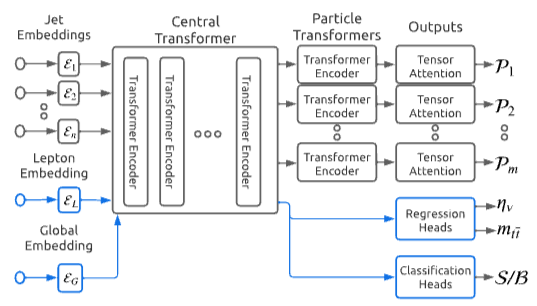
\includegraphics[width=0.8\textwidth]{SPANet2_structure.png}
		\caption{The model structure of SPANet2.}
		\label{fig:SPANet2_structure}
	\end{figure}
% section spanet_classifier (end)
\section{SPANet2 classification}% (fold)
\label{sec:spanet2_classification}
	This section turns off the jet assignment part in SPANet2 by setting the assignment loss weight to zero.
	\begin{itemize}
		\item \verb+assignment_loss_scale+: 0.0
		\item \verb+classification_loss_scale+: 1.0
	\end{itemize}

	Using the mixing $\kappa$ samples for training. The samples are the same as Sec. \ref{subs:training_samples}. Table \ref{tab:SPANET_no_pairing_cls_results} presents the classification training results.
	\begin{table}[htpb]
		\centering
		\caption{The SPANet2 classification training results with mixing $\kappa_\lambda$ sample. The jet assignment part is turned off. The average and standard deviation of 10 training are presented.}
		\label{tab:SPANET_no_pairing_cls_results}
		\begin{tabular}{c|cc}
		Training sample        & ACC     & AUC   \\ \hline
		Mixing $\kappa_\lambda $ & $0.809 \pm 0.013$ & $0.890 \pm 0.014$
		\end{tabular}      
	\end{table}

	Set $p_\text{th} = 0.93$ and use the profile likelihood method and CLs method for the $\kappa_\lambda$ setting. Table \ref{tab:kappa_constraint_SPANet_no_pair} is the results of $\kappa_\lambda$ constraints. These results are worse than simultaneously training on jet assignment and classification tasks.
	\begin{table}[htpb]
		\centering
		\caption{The $\kappa_\lambda$ constraints of SPANet2.}
		\label{tab:kappa_constraint_SPANet_no_pair}
		\begin{tabular}{c|cc|cc}
							  & \multicolumn{4}{c}{Expected Constraint}                          \\
							  & \multicolumn{2}{c}{Profile likelihood} & \multicolumn{2}{c}{CLs} \\ \hline
		Selection method      & Lower              & Upper             & Lower      & Upper      \\ \hline
		SPANet2      & $-5.01$            & $10.97$             & $-4.92$      & $10.89$      \\
		\end{tabular}
	\end{table}
% section spanet2_classification (end)	
\section{SPANet embedding vectors}% (fold)
\label{sec:spanet_embedding_vectors}
	The SPANet embedding vectors can be saved in \verb+.hdf5+ file by this command
	\begin{verbatim}
		python -m spanet.predict <log_dir> <output name> -tf <TEST_FILE> \
		--gpu --output_vectors
	\end{verbatim}
	\verb+<log_dir>+: directory containing the checkpoint and options file. \verb+<TEST_FILE>+: the test file path.

	\subsection{Principal component analysis}% (fold)
	\label{sub:principal_component_analysis}
		Use the PCA class implemented in scikit-learn to do the principal component analysis (PCA) on the SPANet embedding vectors. The variance ratio of the first ten components is shown in Figure \ref{fig:PCA_variance_ratio}.
		\begin{figure}[htpb]
			\centering
			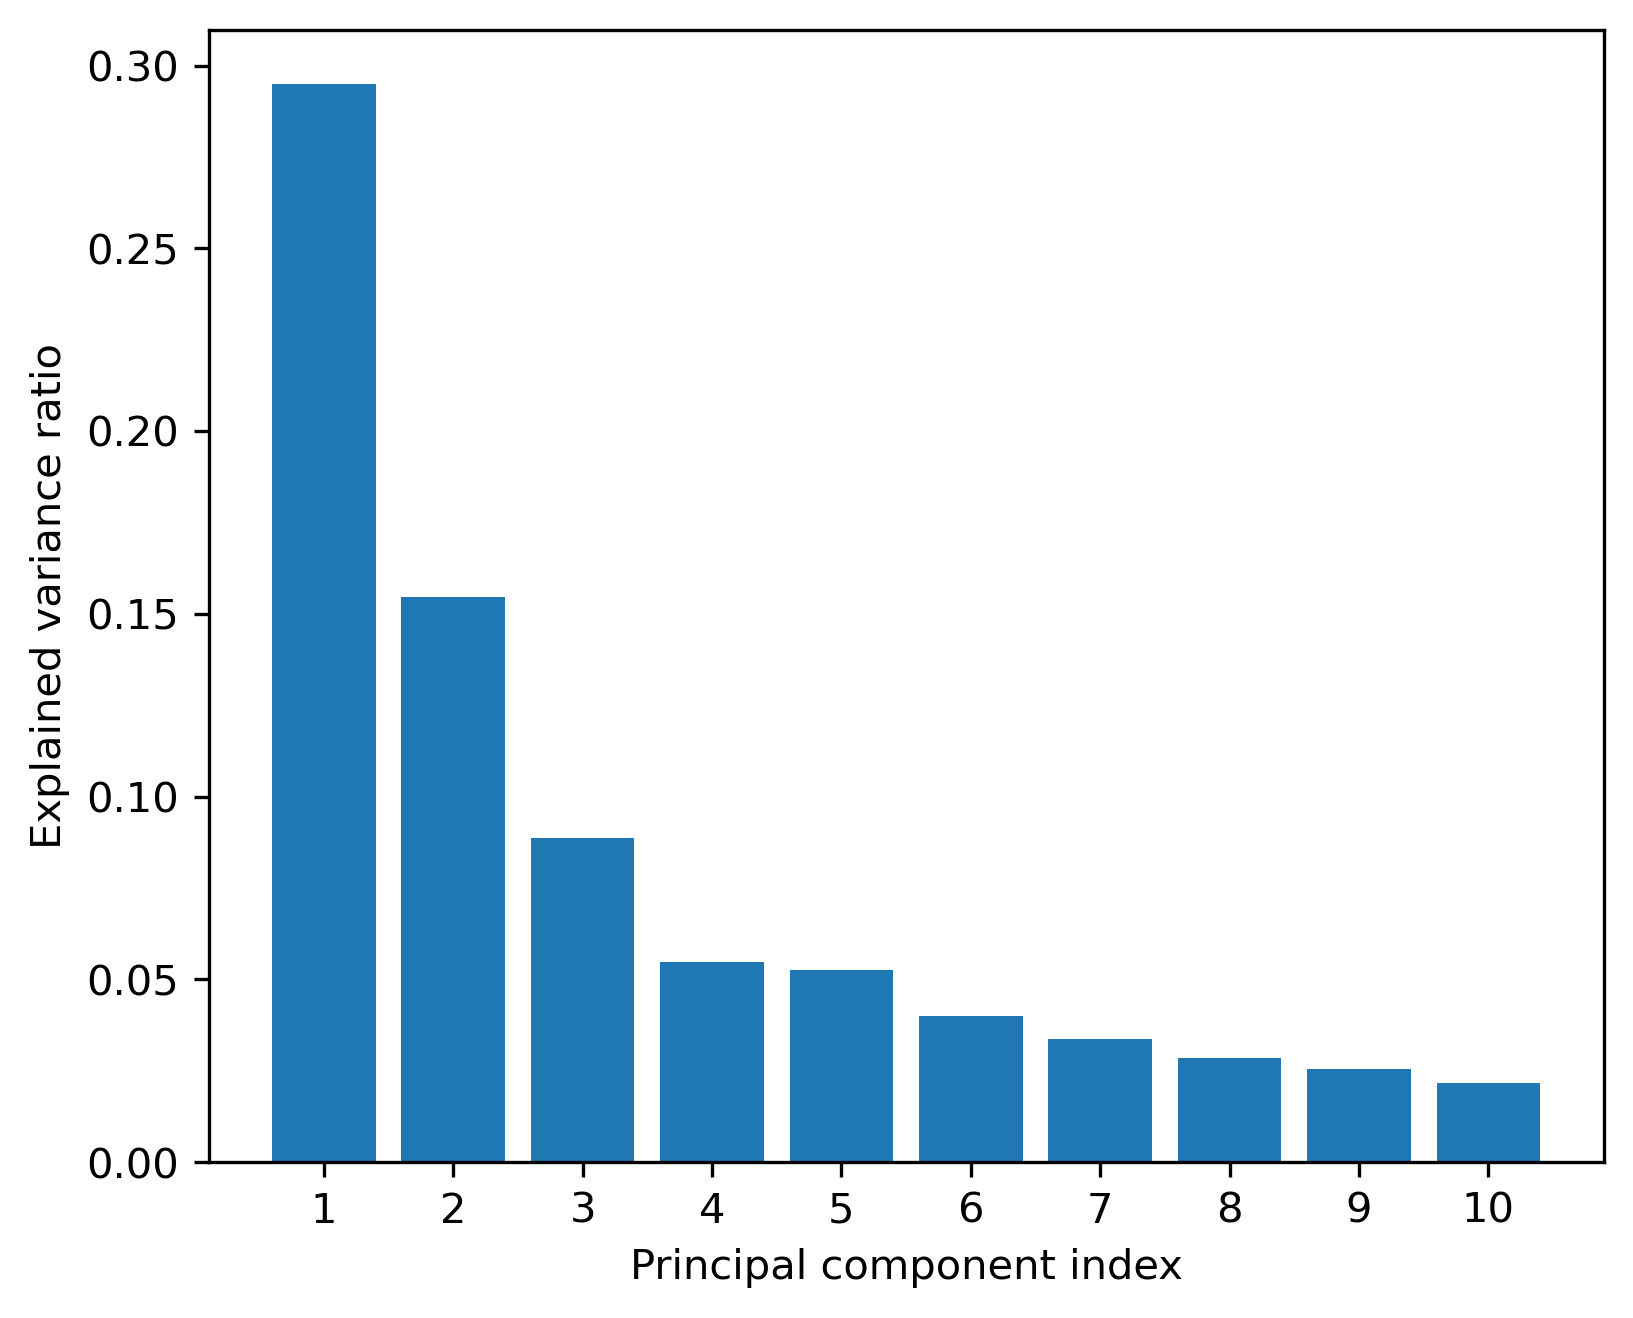
\includegraphics[width=0.7\textwidth]{PCA_variance_ratio.png}
			\caption{The variance ratio of the first ten principal components.}
			\label{fig:PCA_variance_ratio}
		\end{figure}

		Calculate the correlation coefficients with principal components and the high-level observables. The high-level observables are the DNN input features that are constructed by the SPANet2 pairing.

		The results are presented in Figure \ref{fig:correlation_coefficients_pca}. In Figure \ref{fig:correlation_coefficients_pca-signal-background}, the correlation coefficients of signal and background events are calculated separately. The level of correlation of most variables is very low in the background case compared to the signal one's.
		\begin{figure}[htpb]
			\centering
			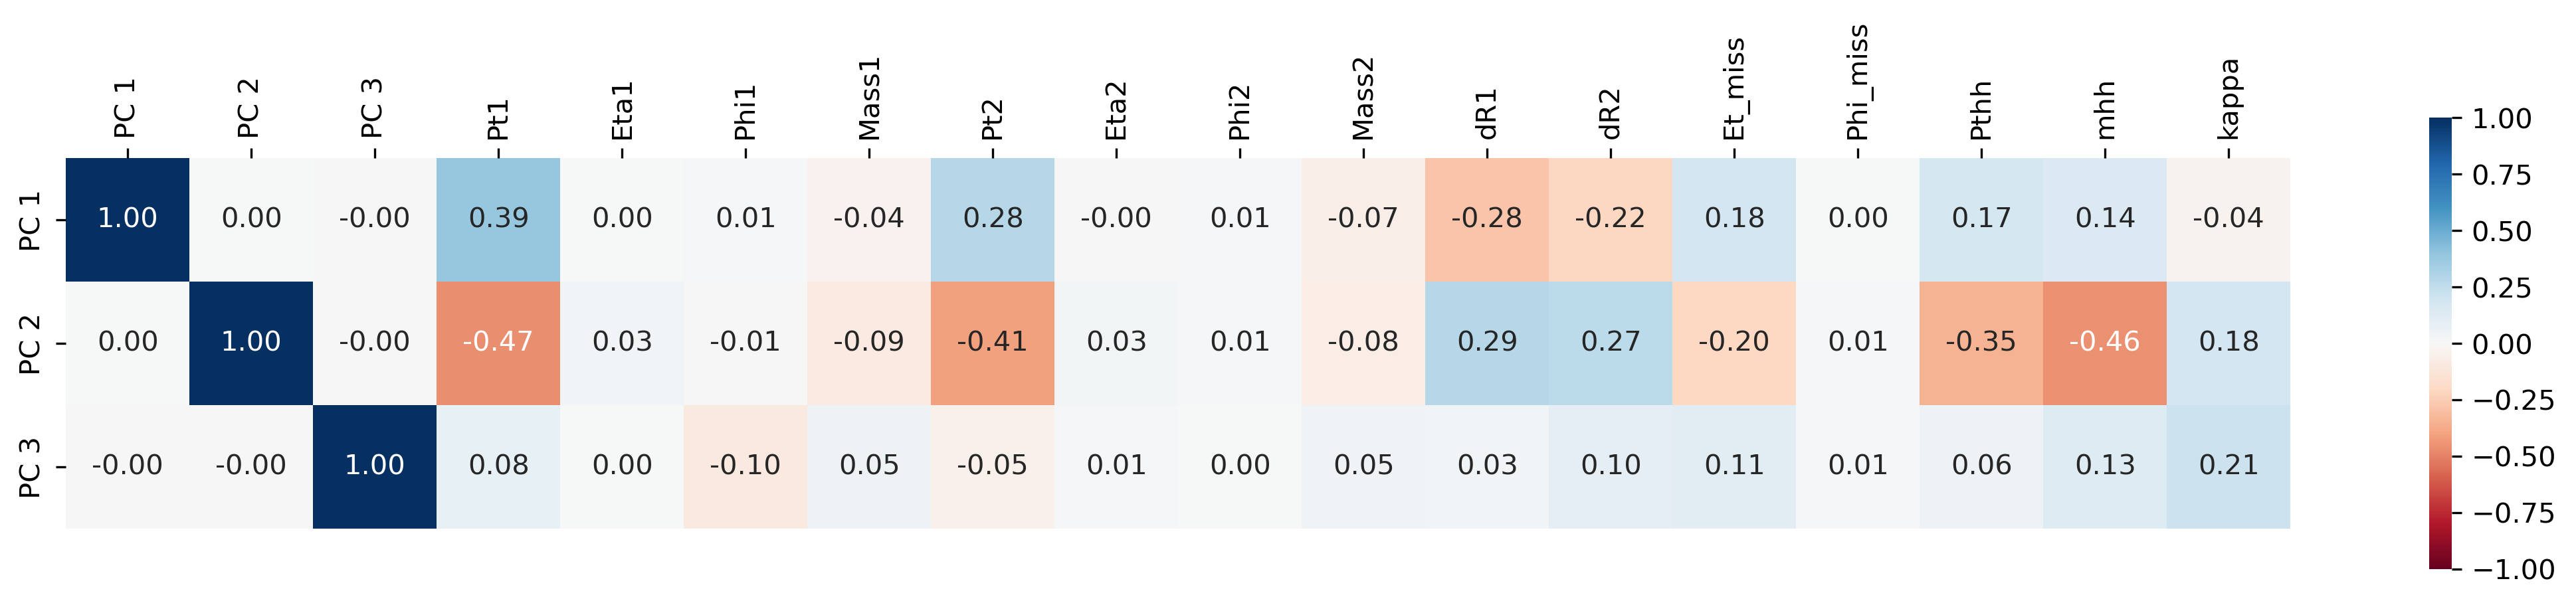
\includegraphics[width=0.99\textwidth]{correlation_coefficients_pca.png}
			\caption{The correlation coefficients of the first three principal components and high-level observables.}
			\label{fig:correlation_coefficients_pca}
		\end{figure}
		\begin{figure}[htpb]
			\centering
			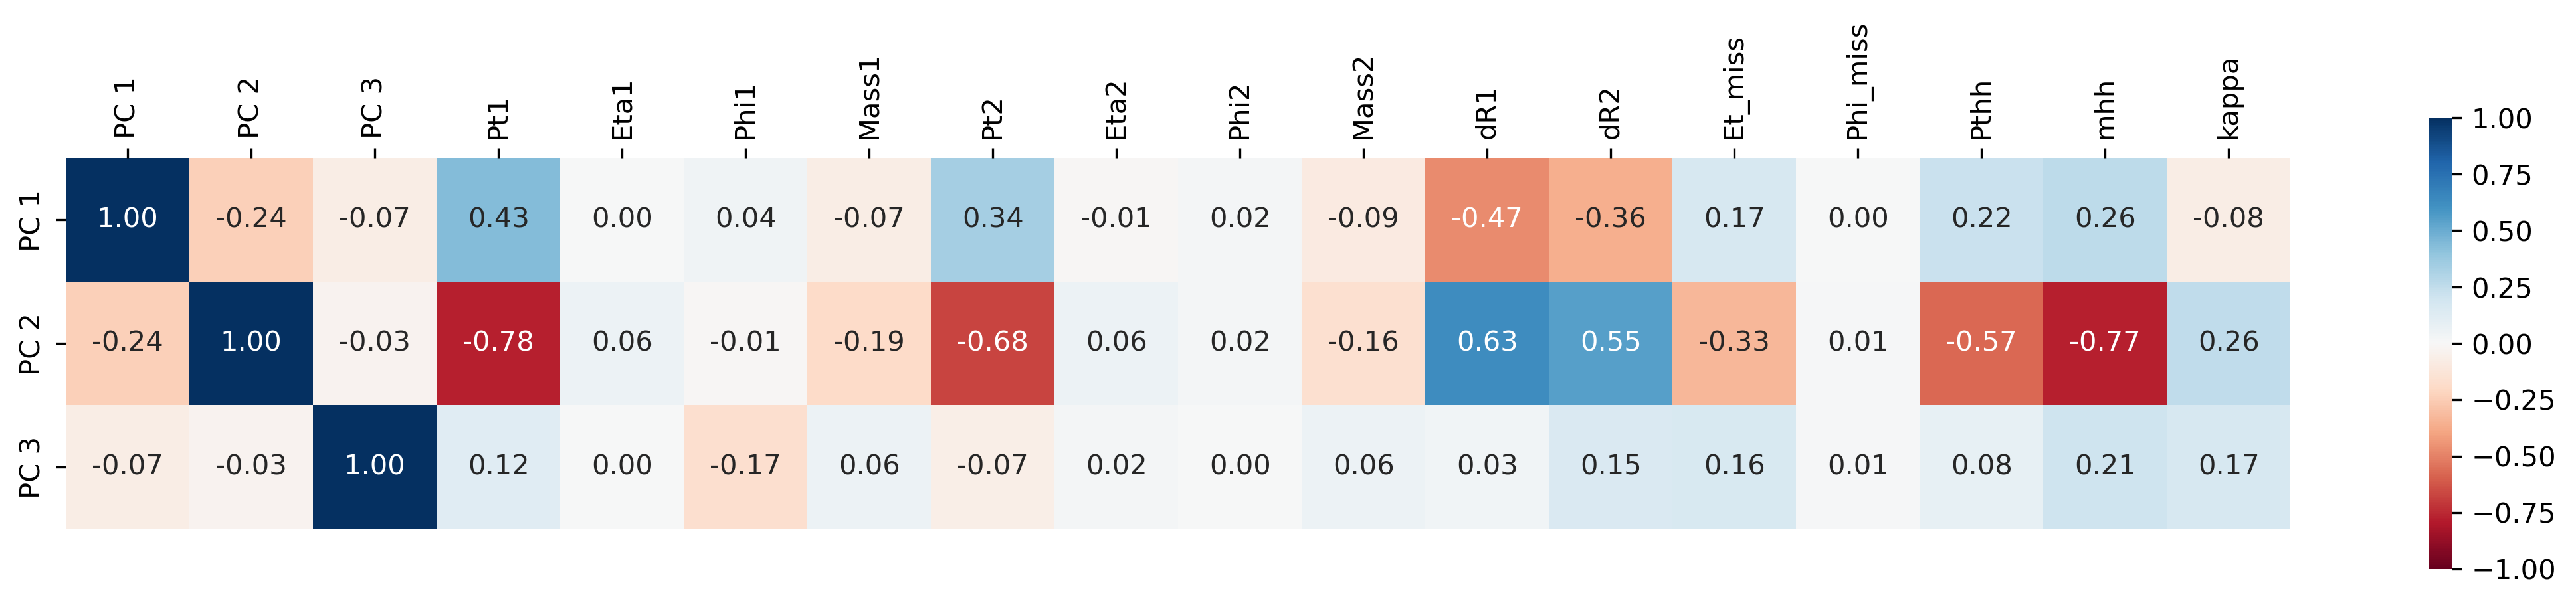
\includegraphics[width=0.99\textwidth]{correlation_coefficients_pca-signal.png}
			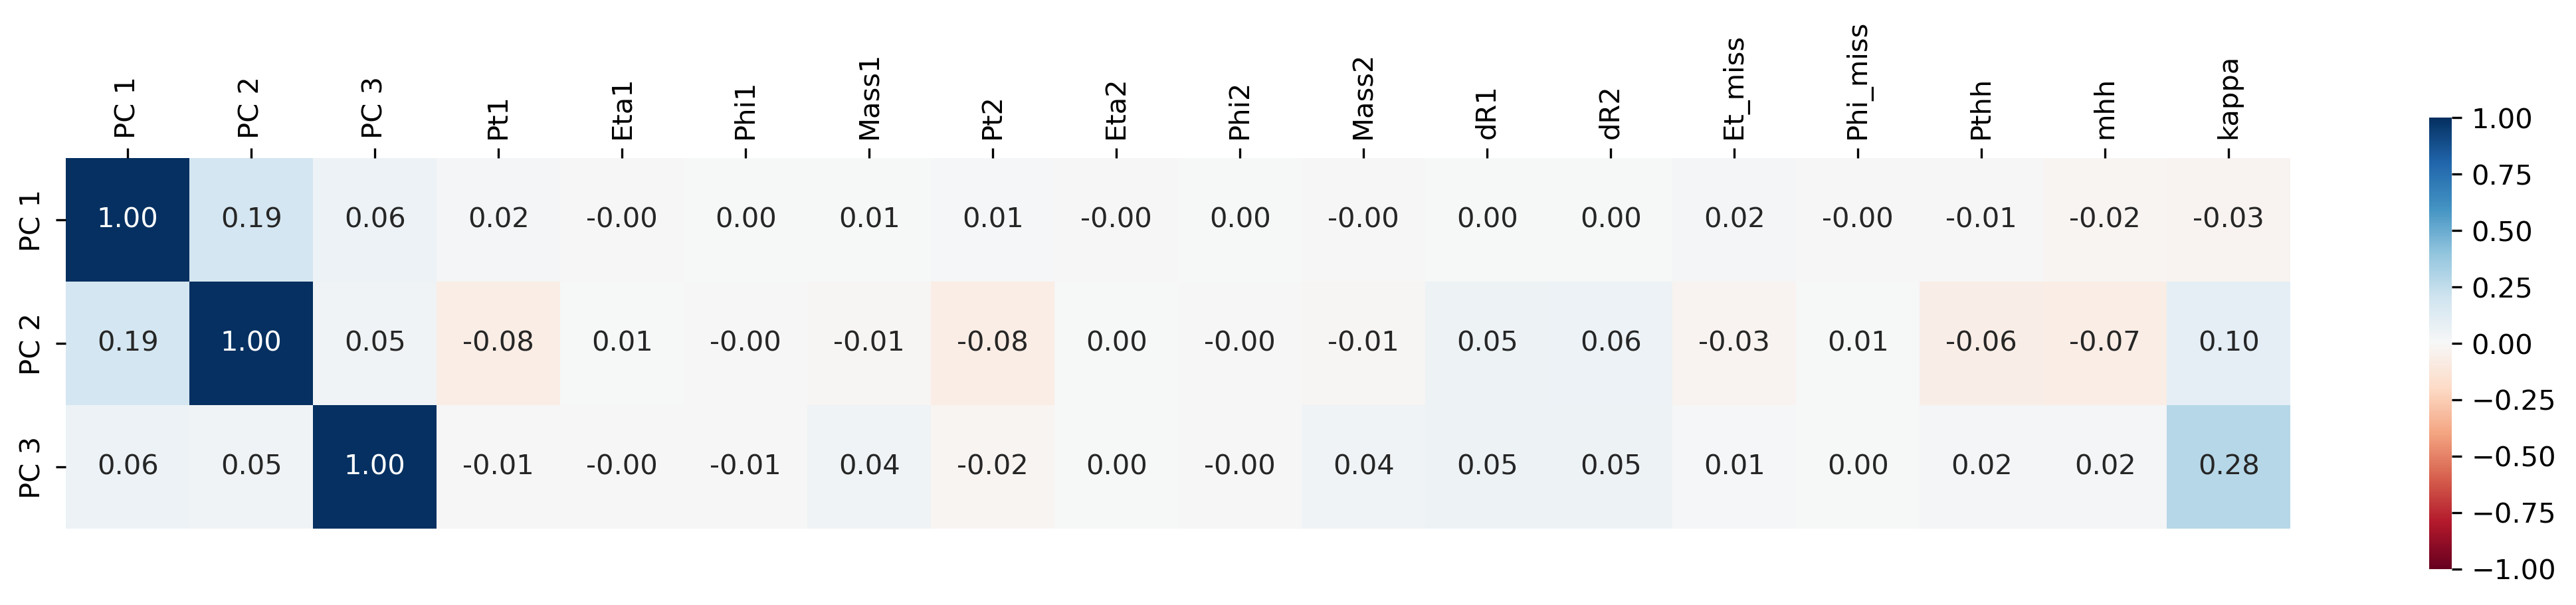
\includegraphics[width=0.99\textwidth]{correlation_coefficients_pca-background.png}
			\caption{The correlation coefficients of the first three principal components and high-level observables. Where the signal and background samples are calculated separately.}
			\label{fig:correlation_coefficients_pca-signal-background}
		\end{figure}

	% subsection principal_component_analysis (end)	
% section spanet_embedding_vectors (end)	
\section{Hyperparameter tuning}% (fold)
\label{sec:hyperparameter_tuning}
	This section uses Optuna to do the hyperparameter optimization.

	\subsection{Optimization range}% (fold)
	\label{sub:optimization_range}
		The optimization range of different hyperparameters is listed in the below
		\begin{itemize}
			\item \verb+learning_rate+: $[10^{-5}, 10^{-2}]$ 
			\item \verb+dropout+: $[0, 0.5]$ 
			\item \verb+gradient_clip+: $[0, 0.5]$ 
			\item \verb+l2_penalty+: $[0, 0.0005]$ 
			\item \verb+hidden_dim+: $[16,32,64,128,256]$ 
			\item \verb+num_encoder_layers+: $[2,8]$ 
			\item \verb+num_branch_encoder_layers+: $[2,8]$ 
			\item \verb+num_classification_layers+: $[1,5]$ 
		\end{itemize}
		Each parameter set was trained for 10 epochs. Test 100 trials.
	% subsection optimization_range (end)
	\subsection{Hyperparameter optimization results}% (fold)
	\label{sub:hyperparameter_optimization_results}
		The hyperparameters optimization results are listed the below
		\begin{itemize}
			\item \verb+learning_rate+: $0.00659$ 
			\item \verb+dropout+: $0.0059$ 
			\item \verb+gradient_clip+: $0.425$ 
			\item \verb+l2_penalty+: $0.000374$ 
			\item \verb+hidden_dim+: $32$ 
			\item \verb+num_encoder_layers+: $8$ 
			\item \verb+num_branch_encoder_layers+: $2$ 
			\item \verb+num_classification_layers+: $1$ 
		\end{itemize}

		Use this parameter set for full training. The samples are the same as Sec. \ref{subs:training_samples}. Table \ref{tab:SPANET_best_hp_cls_results} presents the classification training results. This result is a little better than Table \ref{tab:classification_results_summary2}.
	\begin{table}[htpb]
		\centering
		\caption{The SPANet2 classification training results with mixing $\kappa_\lambda$ sample. Use the Optuna hyperparameter optimization results. The average and standard deviation of 10 training are presented.}
		\label{tab:SPANET_best_hp_cls_results}
		\begin{tabular}{c|cc}
		& ACC     & AUC   \\ \hline
		Best HP & $0.828 \pm 0.002$ & $0.911 \pm 0.001$
		\end{tabular}      
	\end{table}

	Set $p_\text{th} = 0.95$ and use the profile likelihood method and CLs method for the $\kappa_\lambda$ setting. Table \ref{tab:kappa_constraint_SPANet_best_hp} is the results of $\kappa_\lambda$ constraints. These results are similar to the previous one (Table \ref{tab:kappa_constraint_summary2}).
	\begin{table}[htpb]
		\centering
		\caption{The $\kappa_\lambda$ constraints of SPANet2.}
		\label{tab:kappa_constraint_SPANet_best_hp}
		\begin{tabular}{c|cc|cc}
							  & \multicolumn{4}{c}{Expected Constraint}                          \\
							  & \multicolumn{2}{c}{Profile likelihood} & \multicolumn{2}{c}{CLs} \\ \hline
		Selection method      & Lower              & Upper             & Lower      & Upper      \\ \hline
		SPANet2      & $-3.07$            & $8.80$             & $-3.04$      & $8.76$      \\
		\end{tabular}
	\end{table}

	% subsection hyperparameter_optimization_results (end)	
	\subsection{DNN hyperparameter optimization}% (fold)
	\label{sub:dnn_hyperparameter_optimization}
		The optimization range of different hyperparameters is listed in the below
		\begin{itemize}
			\item \verb+learning_rate+: $[10^{-5}, 10^{-1}]$ 
			\item \verb+hidden_dim+: $[16,32,64,128,256]$ 
			\item \verb+n_layers+: $[1,5]$ 
		\end{itemize}
		Test 100 trials.
	% subsection dnn_hyperparameter_optimization (end)
	\subsection{DNN hyperparameter optimization results}% (fold)
	\label{sub:dnn_hyperparameter_optimization_results}
		For $\text{min-}\Delta R$, the hyperparameters optimization results are 
		\begin{itemize}
			\item \verb+learning_rate+: $0.00495$ 
			\item \verb+hidden_dim+: $256$ 
			\item \verb+n_layers+: $3$ 
		\end{itemize}
		
		For mixing $\kappa$ SPANet2, the results are
		\begin{itemize}
			\item \verb+learning_rate+: $0.000948$ 
			\item \verb+hidden_dim+: $256$ 
			\item \verb+n_layers+: $2$ 
		\end{itemize}

		Use these parameter sets for training. The samples are the same as Sec. \ref{sub:training_samples2}. Table \ref{tab:DNN_best_hp_cls_results} presents the DNN classification training results. The results are similar to Table \ref{tab:classification_results_summary2}.
		\begin{table}[htpb]
			\centering
			\caption{The DNN classification training results with mixing $\kappa_\lambda$ sample. Use the Optuna hyperparameter optimization results. The average and standard deviation of 10 training are presented.}
			\label{tab:DNN_best_hp_cls_results}
			\begin{tabular}{c|cc}
				& ACC     & AUC   \\ \hline
				$\text{min-}\Delta R$   & $0.799 \pm 0.011$ & $0.881 \pm 0.012$ \\
				mixing $\kappa$ SPANet2 & $0.803 \pm 0.004$ & $0.884 \pm 0.004$
			\end{tabular}      
		\end{table}

		Set $p_\text{th} = 0.95$ and use the profile likelihood method and CLs method for the $\kappa_\lambda$ setting. Table \ref{tab:kappa_constraint_DNN_best_hp} is the results of $\kappa_\lambda$ constraints. These results are similar to the previous one (Table \ref{tab:kappa_constraint_summary2}).
		\begin{table}[htpb]
			\centering
			\caption{The $\kappa_\lambda$ constraints of DNN with best hyperparameters.}
			\label{tab:kappa_constraint_DNN_best_hp}
			\begin{tabular}{c|cc|cc}
								  & \multicolumn{4}{c}{Expected Constraint}                          \\
								  & \multicolumn{2}{c}{Profile likelihood} & \multicolumn{2}{c}{CLs} \\ \hline
			Selection method      & Lower              & Upper             & Lower      & Upper      \\ \hline
			$\text{min-}\Delta R$ DNN   & $-3.20$            & $10.31$            & $-3.16$      & $10.19$      \\
			mixing $\kappa$ SPANet2 DNN & $-3.29$            & $11.14$            & $-3.14$      & $11.04$      \\
			\end{tabular}
		\end{table}
	% subsection dnn_hyperparameter_optimization_results (end)	
% section hyperparameter_tuning (end)		
\section{Summary}% (fold)
\label{sec:summary2}
	\subsection{Pairing performance}% (fold)
	\label{sub:pairing_performance2}
	Figure \ref{fig:pairing_performance_kappa2} shows the pairing efficiency of different methods. Table \ref{tab:pairing_performance_kappa} is the pairing efficiency of some $\kappa_\lambda$ points. Where the mixing $\kappa$ SPANet2 has the best performance.
		\begin{table}[htpb]
			\centering
			\caption{The classification performance of different selection methods.}
			\label{tab:pairing_performance_kappa}
			\begin{tabular}{l|ccc}
			& \multicolumn{3}{c}{$\kappa_\lambda$} \\
			Pairing method          & $-5$    & $1$     & $5$  \\ \hline
			$\text{min-}\Delta R$ 	& $0.644$ & $0.809$ & $0.395$  \\
			mixing $\kappa$ SPANet2 & $0.793$ & $0.885$ & $0.729$
			\end{tabular}			
		\end{table}

		\begin{figure}[htpb]
			\centering
			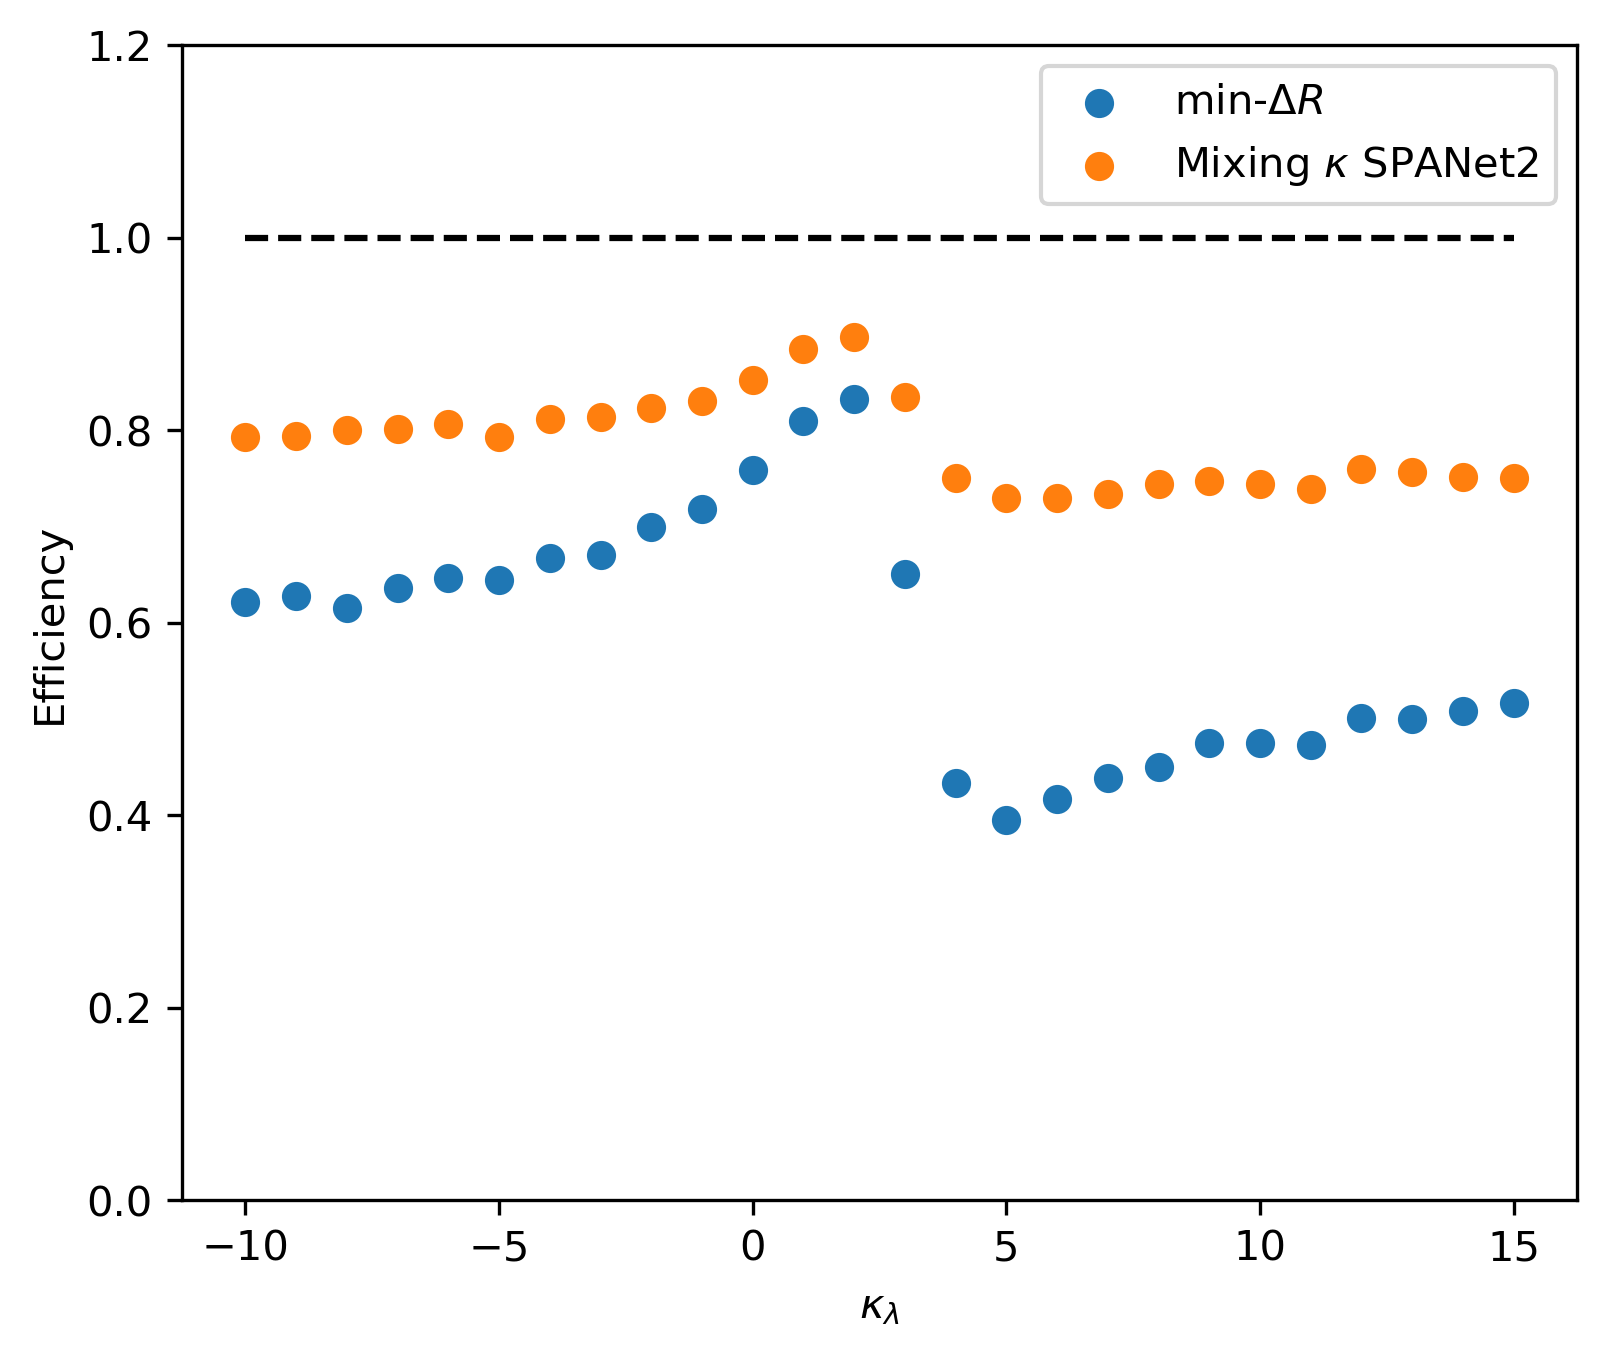
\includegraphics[width=0.65\textwidth]{pairing_efficiency_kappa-mindR-SPANet2.png}
			\caption{The pairing performance for different $\kappa_\lambda$ samples.}
			\label{fig:pairing_performance_kappa2}
		\end{figure}

	% subsection pairing_performance (end)
	\subsection{Classification performance}% (fold)
	\label{sub:classification_performance_summary2}
		Table \ref{tab:classification_results_summary3} presents the classification training results. Where the hyperparameter optimization is finished.
		\begin{table}[htpb]
			\centering
			\caption{The classification performance of different selection methods.}
			\label{tab:classification_results_summary3}
			\begin{tabular}{l|cc}
			Selection method          & ACC   & AUC   \\ \hline
			$\text{min-}\Delta R$ DNN   & $0.799 \pm 0.011$ & $0.881 \pm 0.012$ \\
			mixing $\kappa$ SPANet2 DNN & $0.803 \pm 0.004$ & $0.884 \pm 0.004$ \\
			mixing $\kappa$ SPANet2     & $0.828 \pm 0.002$ & $0.911 \pm 0.001$ 
			\end{tabular}			
		\end{table}
	% subsection classification_performance (end)
	\subsection{\texorpdfstring{$\kappa_\lambda$}{kappa} constraints}% (fold)
	\label{sub:kappa_constraints2}
		Table \ref{tab:kappa_constraint_summary3} is the $\kappa_\lambda$ constraints of the different selection methods. Where the hyperparameter optimization is finished.
		\begin{table}[htpb]
			\centering
			\caption{The $\kappa_\lambda$ constraints of different selection methods.}
			\label{tab:kappa_constraint_summary3}
			\begin{tabular}{cc|cc|cc}
									&                  & \multicolumn{4}{c}{Expected Constraints}                         \\
									&                  & \multicolumn{2}{c}{Profile likelihood} & \multicolumn{2}{c}{CLs} \\ \hline
			Pairing method          & Selection method & Lower              & Upper             & Lower       & Upper     \\ \hline
			$\text{min-}\Delta R$   & DNN              & $-3.20$            & $10.31$           & $-3.16$      & $10.19$    \\
			Mixing $\kappa$ SPANet2 & DNN              & $-3.29$            & $11.14$           & $-3.14$      & $11.04$   \\
			Mixing $\kappa$ SPANet2 & SPANet2          & $-3.07$            & $8.80$            & $-3.04$      & $8.76$   
			\end{tabular}		
		\end{table}
	% subsection kappa_constraints (end)
% section summary2 (end)		
\section{Compared 13 TeV and 14 TeV samples}% (fold)
\label{sec:compared_13_tev_and_14_tev_samples}
	This section plots the $p_\text{T}$, $\eta$, and invariant mass distribution with different energy.
	\subsection{Signal plots}% (fold)
	\label{sub:signal_plots}
		Generate the di-Higgs samples with $\sqrt{s} = \text{13 TeV and 14 TeV}$, then plot the total invariant mass of di-Higgs $m_{hh}$ and the $p_{\text{T}}$ of Higgs. The results are presented in Figure \ref{fig:di-Higgs-SM-kappa-13-14TeV}. The distribution of different energy is similar.

		\begin{figure}[htpb]
			\centering
			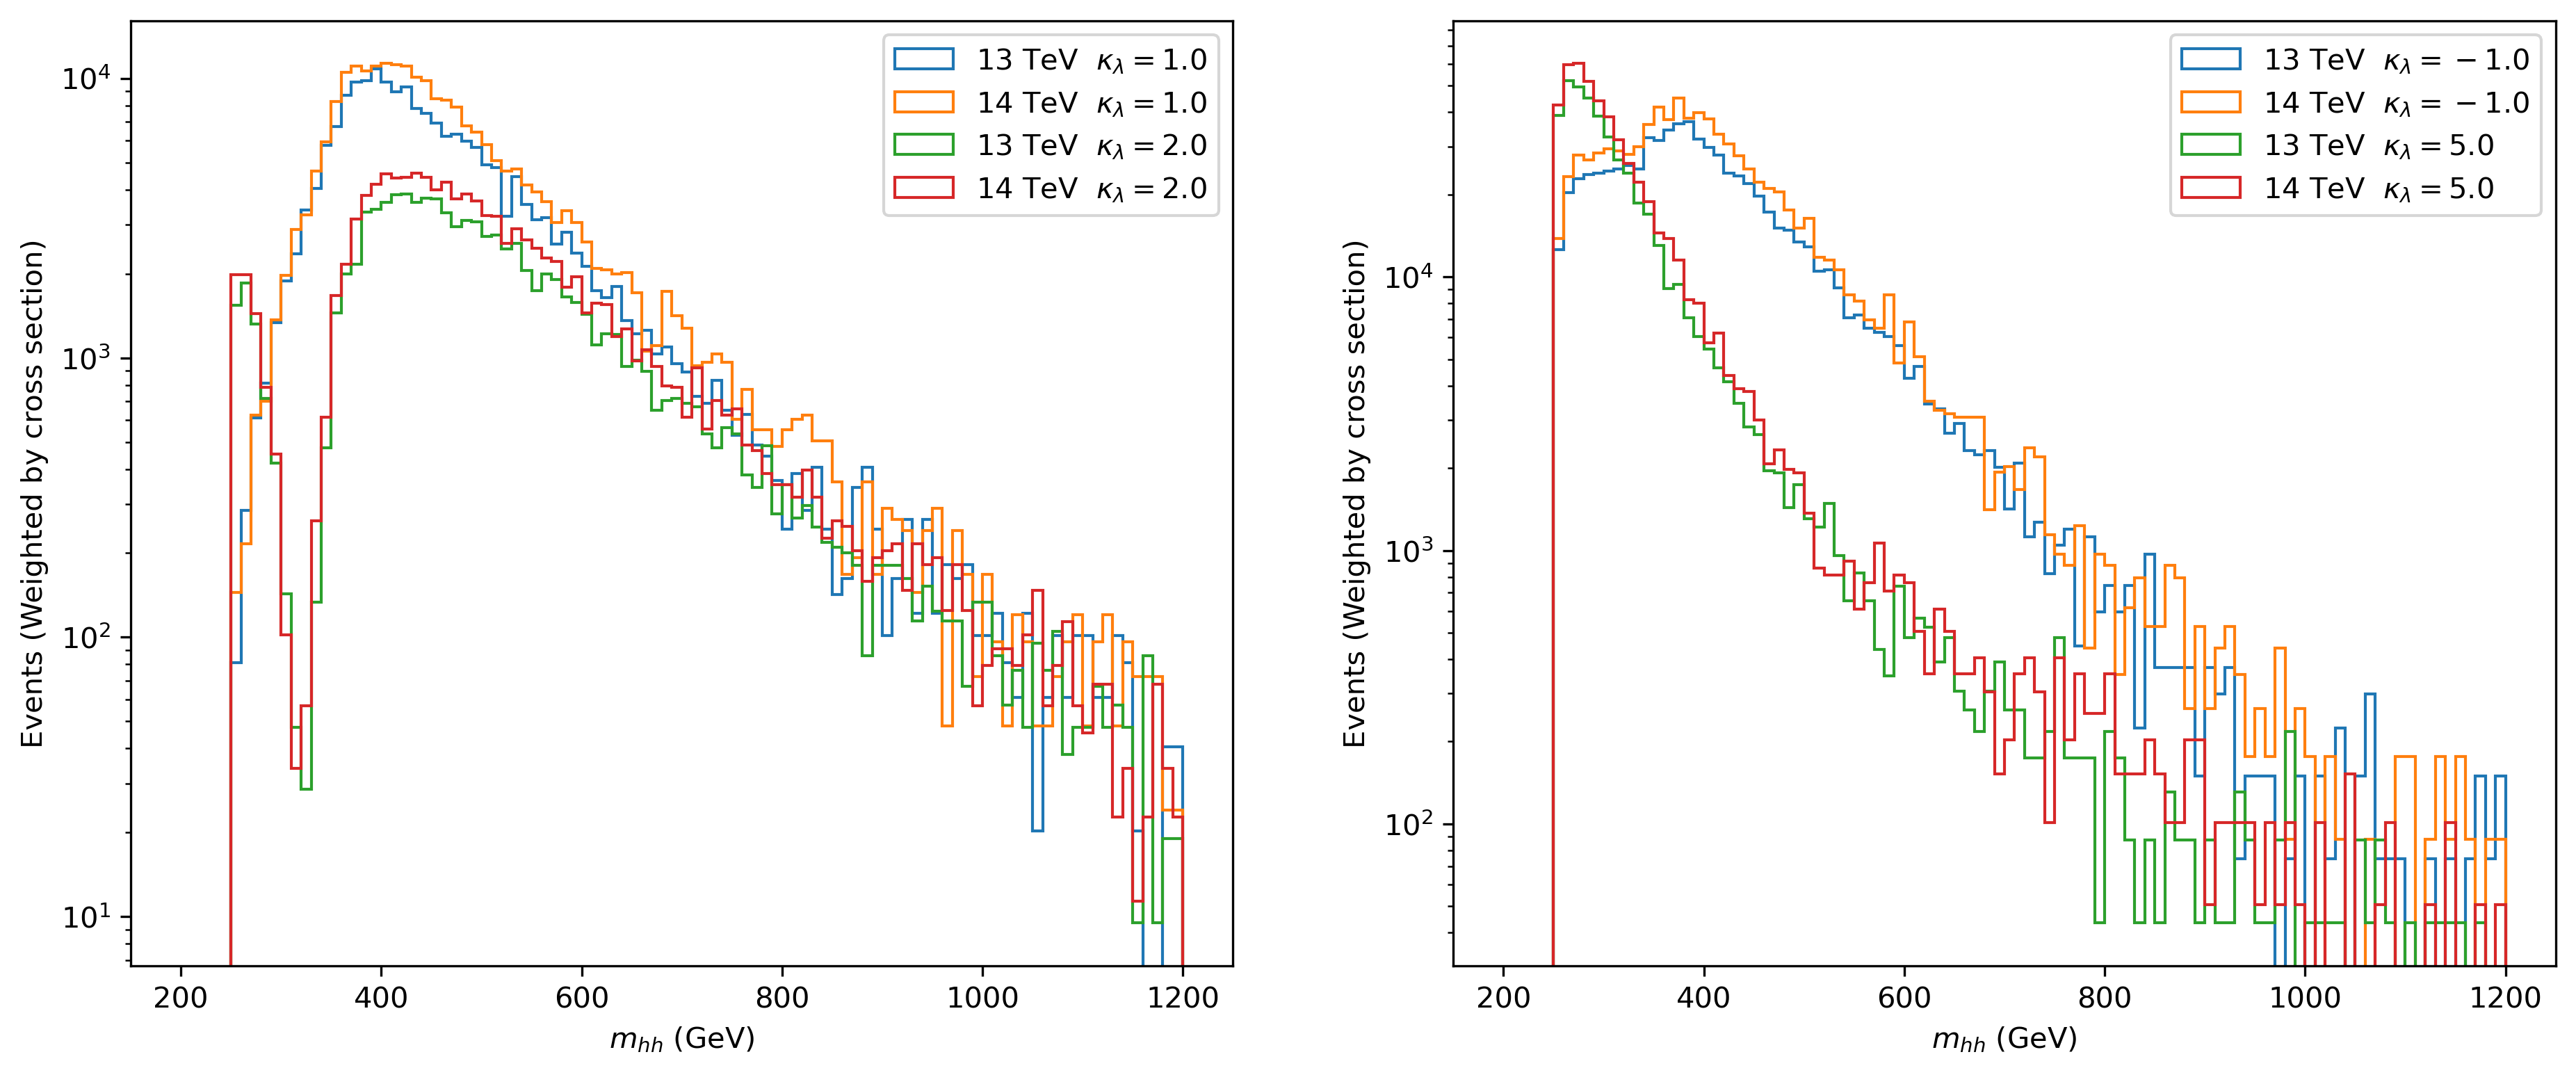
\includegraphics[width=0.9\textwidth]{di-Higgs-SM-kappa-mhh-13-14TeV.png}
			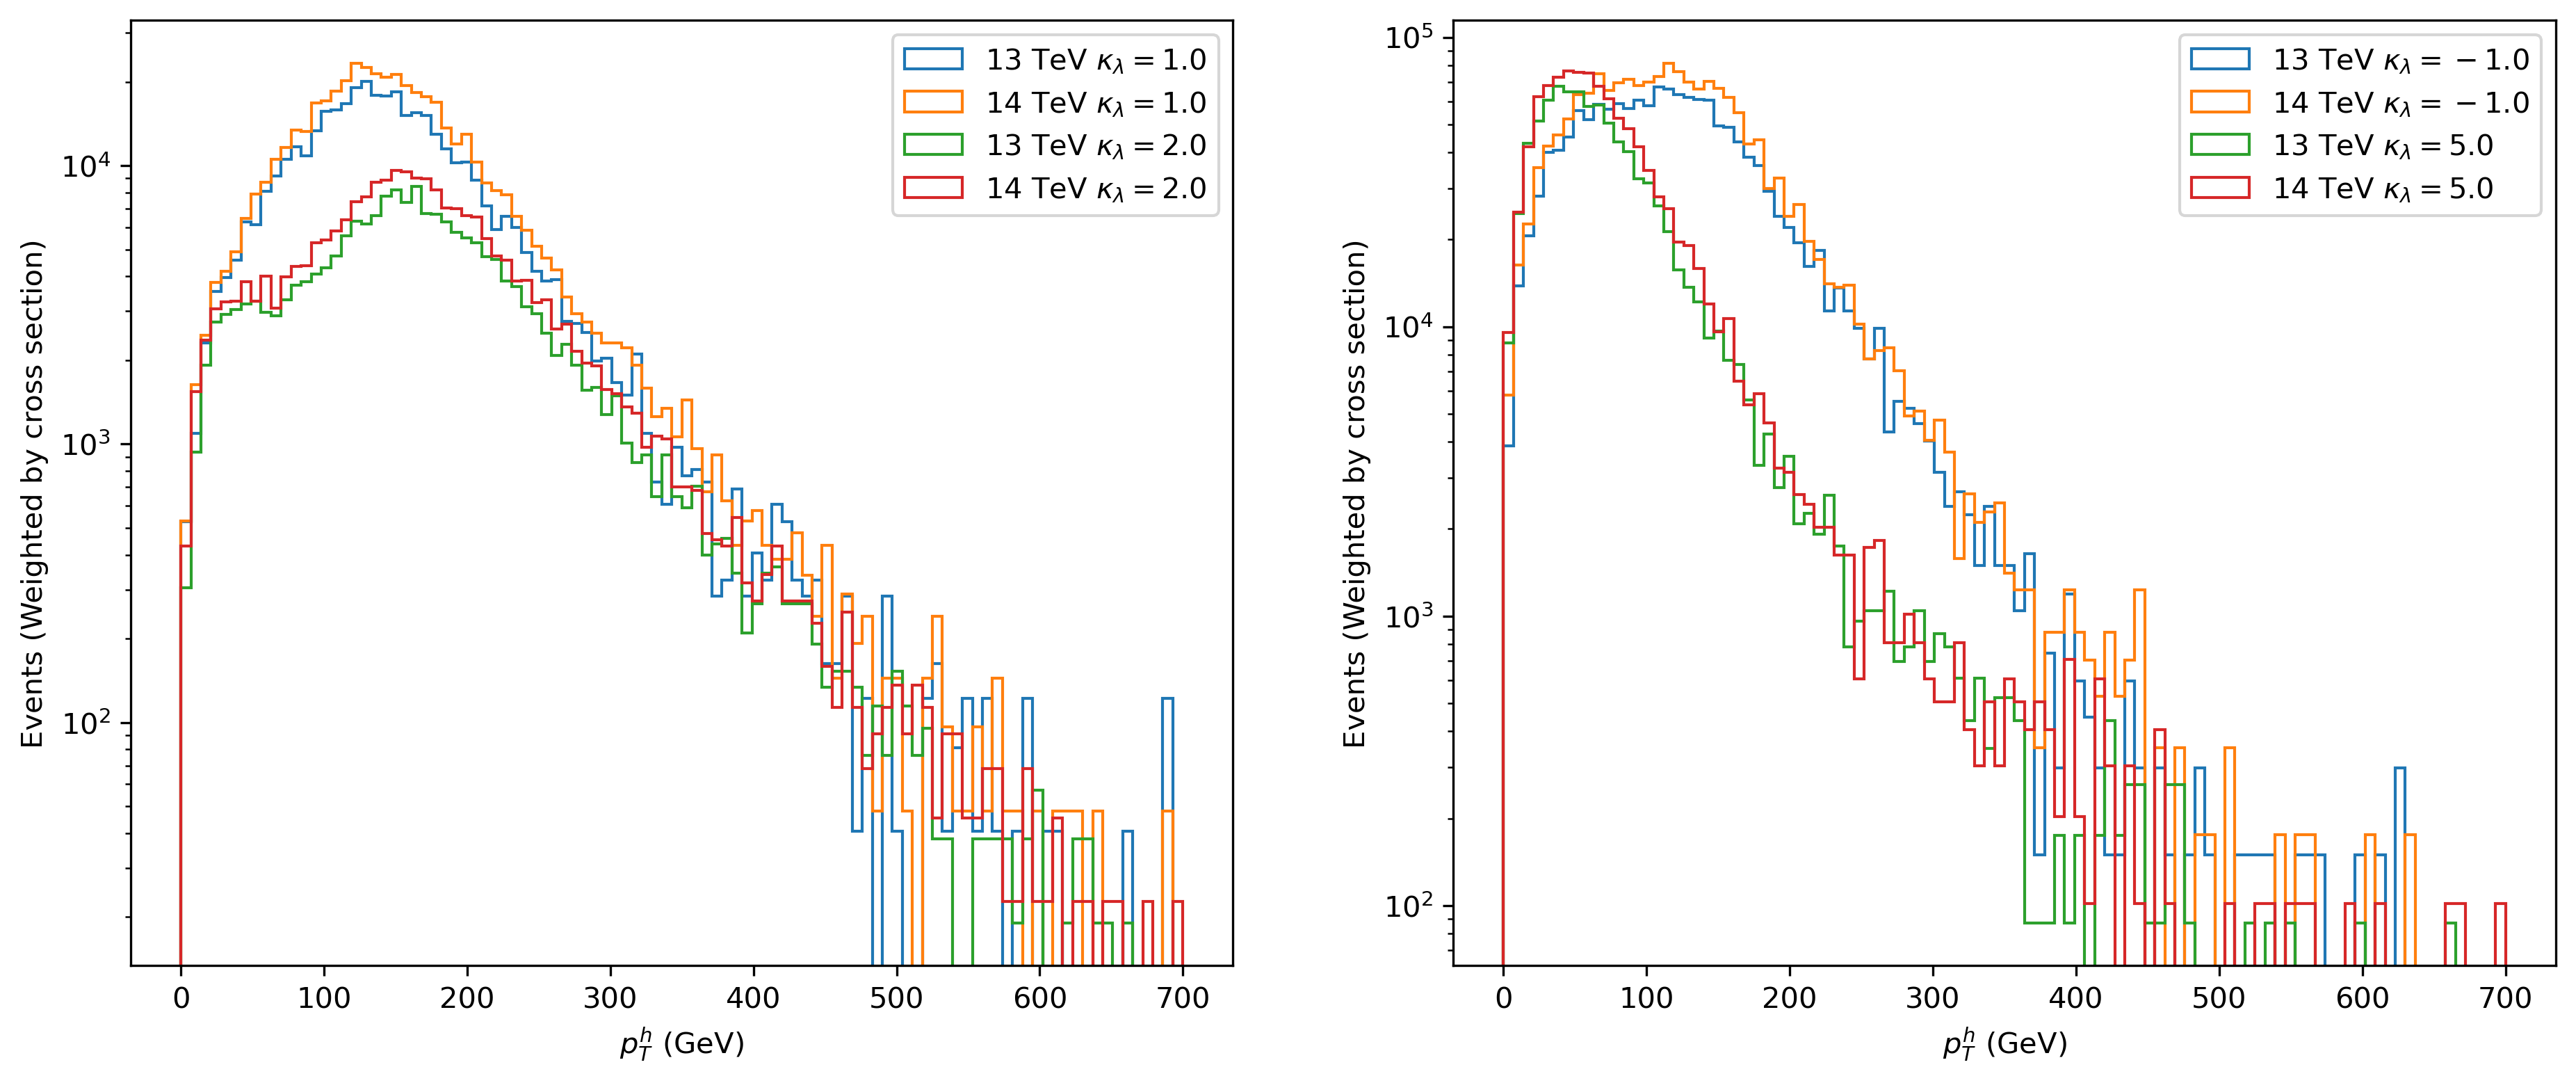
\includegraphics[width=0.9\textwidth]{di-Higgs-SM-kappa-pth-13-14TeV.png}
			\caption{The total invariant mass $m_{hh}$ distribution of di-Higgs system and the $p_{\text{T}}^{h}$ distribution of Higgs. The distribution of different energy look similar.}
			\label{fig:di-Higgs-SM-kappa-13-14TeV}
		\end{figure}
	% subsection signal_plots (end)
	\subsection{Background plots}% (fold)
	\label{sub:background_plots}
	Generate the pp4b samples with $\sqrt{s} = \text{13 TeV and 14 TeV}$, then plot the total invariant mass of 4b quarks and the $p_{\text{T}}$ $\eta$ of b quarks. The results are presented in Figure \ref{fig:pp4b-m4b-13-14TeV} and Figure \ref{fig:pp4b-pt-eta-13-14TeV}. The distribution of different energy is similar.
		\begin{figure}[htpb]
			\centering
			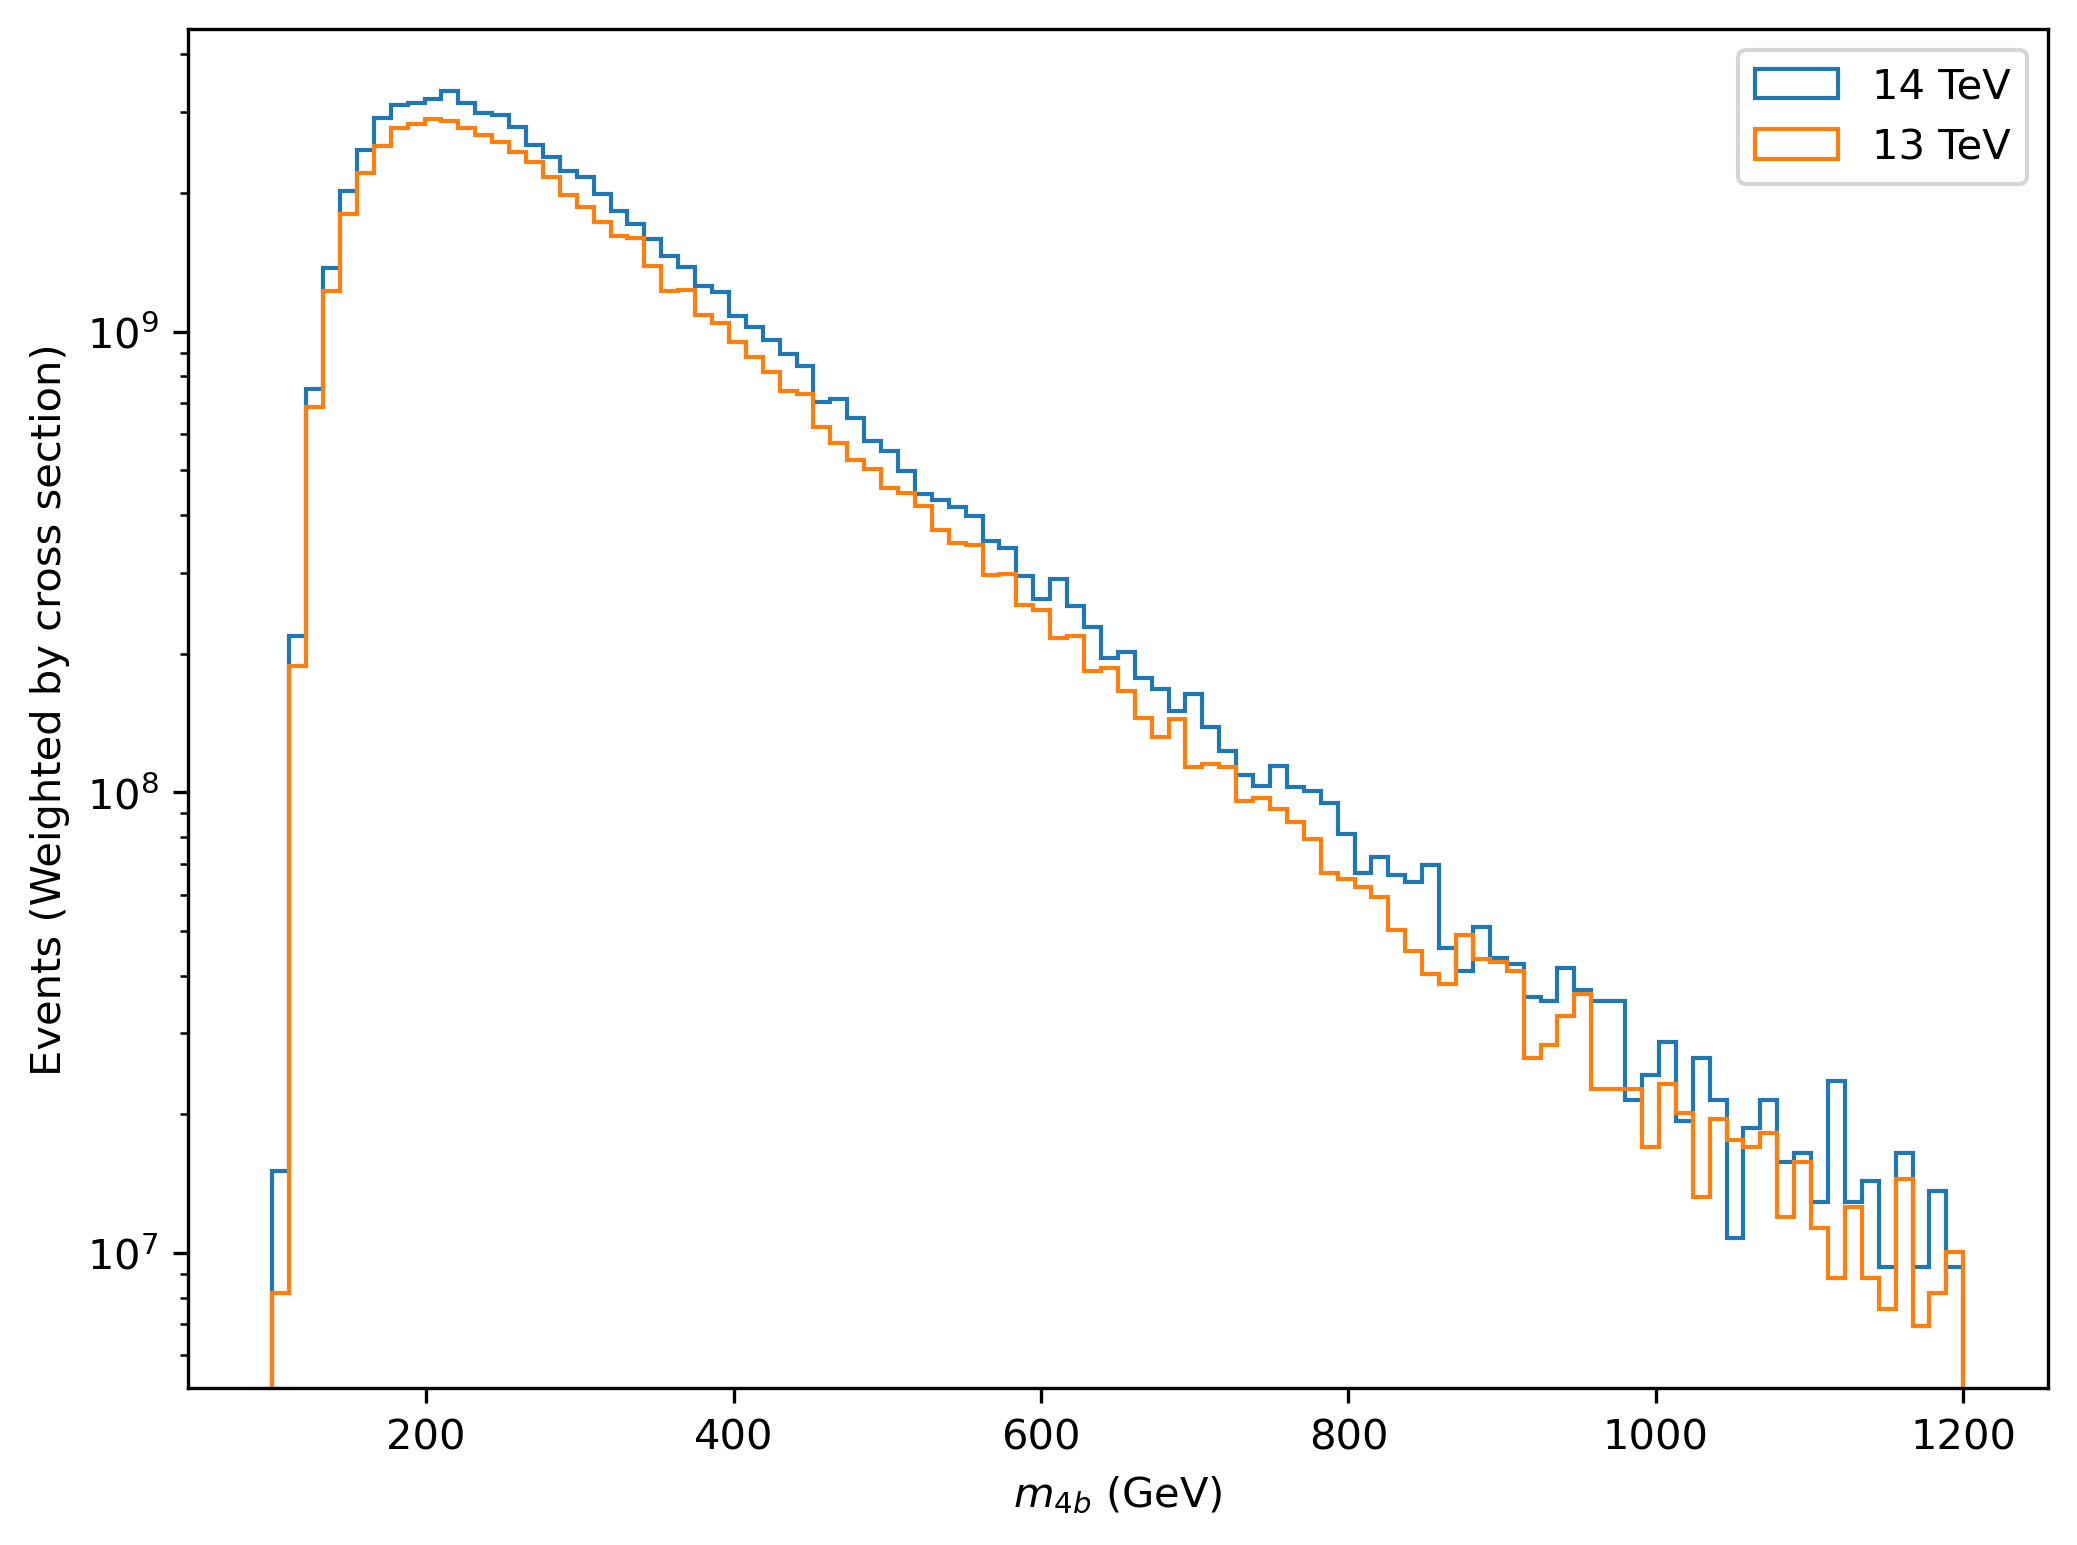
\includegraphics[width=0.6\textwidth]{pp4b-m4b-13-14TeV.png}
			\caption{The total invariant mass $m_{4b}$ distribution}
			\label{fig:pp4b-m4b-13-14TeV}
		\end{figure}

		\begin{figure}[htpb]
			\centering
			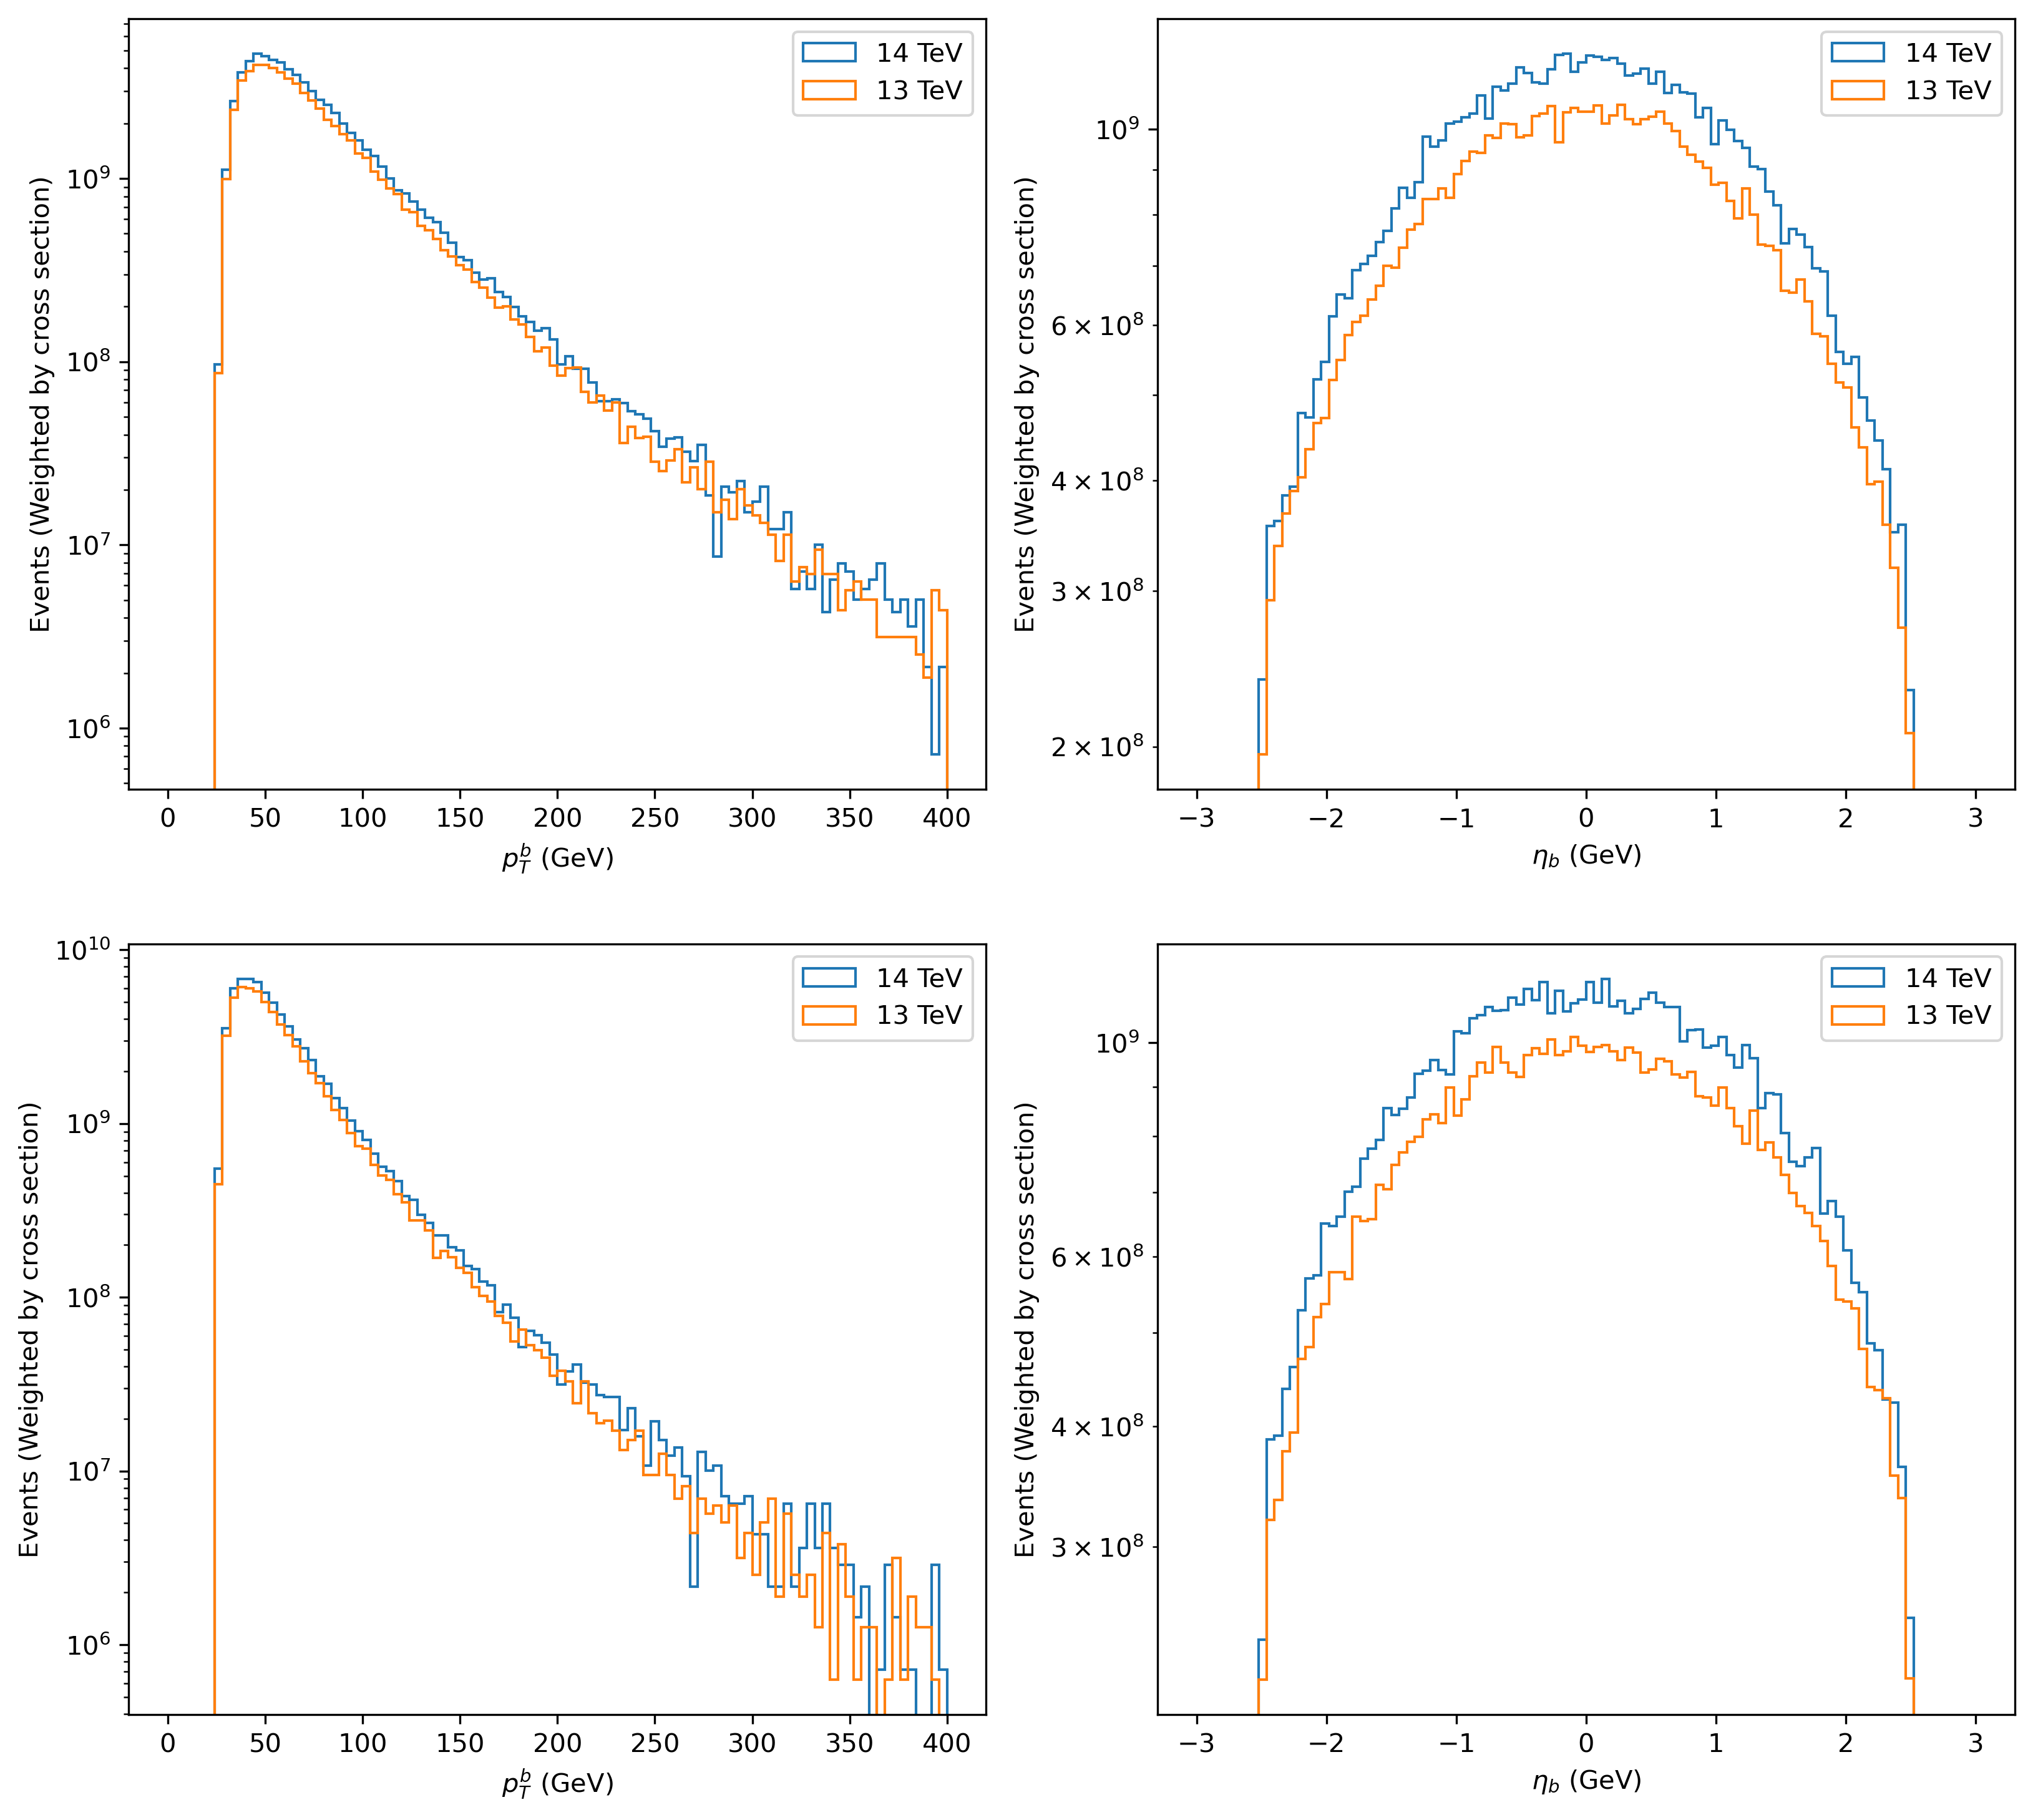
\includegraphics[width=0.9\textwidth]{pp4b-pt-eta-13-14TeV.png}
			\caption{The $p_{\text{T}}$ and $\eta$ distribution of b quarks, the first row is for leading b quarks and the second row is for sub-leading b quarks. The distribution of different energy look similar.}
			\label{fig:pp4b-pt-eta-13-14TeV}
		\end{figure}
	% subsection background_plots (end)	
% section compared_13_tev_and_14_tev_samples (end)		
\end{document} 

